\documentclass[12pt, a4paper]{article}

% ── Packages ──────────────────────────────────────────────────────────────────
\usepackage[margin=2.5cm]{geometry}
\usepackage{graphicx}
\usepackage{booktabs}
\usepackage{caption}
\usepackage{subcaption}
\usepackage{amsmath}
\usepackage{float}
\usepackage{array}
\usepackage{xcolor}
\usepackage{multirow}
\usepackage{hyperref}
\usepackage{parskip}
\usepackage{microtype}
\usepackage{enumitem}

\graphicspath{{./}}

\hypersetup{
    colorlinks=true,
    linkcolor=blue!60!black,
    citecolor=blue!60!black,
}

\captionsetup{font=small, labelfont=bf, skip=6pt}

% ── Custom colours ─────────────────────────────────────────────────────────────
\definecolor{headblue}{RGB}{21, 101, 192}
\definecolor{lightgray}{RGB}{245, 245, 245}

% ── Title ─────────────────────────────────────────────────────────────────────
\title{
    \vspace{-1cm}
    {\Large\textbf{Cluster Analysis of Alzheimer's Disease Patients}}\\[6pt]
    {\large Using Brain MRI Features and Clinical Data}\\[4pt]
    {\normalsize OASIS-1 Dataset — $n = 216$ complete-case patients}
}
\author{Areg Karapetian}
\date{\today}

% ══════════════════════════════════════════════════════════════════════════════
\begin{document}
\maketitle
\tableofcontents
\newpage

% ══════════════════════════════════════════════════════════════════════════════
\section{Introduction}

This report presents a cluster analysis of Alzheimer's disease patients from the OASIS-1
cross-sectional dataset. The goal is to discover data-driven patient subgroups that may
correspond to clinically meaningful disease stages, by combining brain MRI image features
with clinical assessments.

Four experimental configurations are compared:
\begin{enumerate}[noitemsep]
    \item \textbf{All 5 images + clinical data} — the full feature set
    \item \textbf{Clinical data only} — baseline without any imaging
    \item \textbf{Images only} — imaging features with no clinical signal
    \item \textbf{Best image pair + clinical} (coronal + sagittal) — a reduced but clean image set
\end{enumerate}

All configurations use $k$-medoids clustering (FasterPAM algorithm).
Two values of $k$ are evaluated ($k=2$ and $k=3$) alongside a data-driven $k$-selection
analysis.

% ══════════════════════════════════════════════════════════════════════════════
\section{Dataset and Preprocessing}

\subsection{OASIS-1 Dataset}
The Open Access Series of Imaging Studies (OASIS-1) is a cross-sectional collection of
416 subjects aged 18–96, including cognitively normal individuals and patients with early
Alzheimer's disease. The Clinical Dementia Rating (CDR) scale is used as the ground-truth
label: $\text{CDR}=0$ (healthy), $0.5$ (very mild dementia), $1$ (mild dementia),
$2$ (moderate dementia).

\subsection{Patient Selection}
Of the 416 subjects, \textbf{216 patients} have complete records for all clinical variables
(Education, SES, MMSE) and are retained for this analysis. All 216 patients have a valid
CDR score.

\subsection{Clinical Features}
Eight clinical features are used:

\begin{table}[H]
\centering
\caption{Clinical features used in experiments.}
\begin{tabular}{llll}
\toprule
\textbf{Feature} & \textbf{Type} & \textbf{Scale} & \textbf{Distance block} \\
\midrule
Age & Continuous & years & p1 (Euclidean) \\
MMSE & Continuous & 0--30 & p1 (Euclidean) \\
eTIV & Continuous & mm$^3$ & p1 (Euclidean) \\
nWBV & Continuous & 0--1 & p1 (Euclidean) \\
ASF & Continuous & ratio & p1 (Euclidean) \\
\midrule
M/F & Nominal binary & M/F & p3 (Hamming) \\
Education & Ordinal & 1--5 & p3 (Hamming) \\
SES & Ordinal & 1--5 & p3 (Hamming) \\
\bottomrule
\end{tabular}
\end{table}

\subsection{Image Features — HOG Pipeline}
Each patient has up to five MRI image types:
\texttt{cor} (coronal), \texttt{gfc\_sag} (sagittal), \texttt{gfc\_tra} (transverse),
\texttt{masked\_tra} (skull-stripped transverse), \texttt{sbj\_sag} (native-space sagittal).

Images are preprocessed with:
\begin{itemize}[noitemsep]
    \item Zero-padding to square using the longest dimension, centred
    \item Resize to $128 \times 128$ pixels
    \item Histogram of Oriented Gradients (HOG): 9 orientations, $8 \times 8$ px/cell,
          $2 \times 2$ cells/block $\Rightarrow$ \textbf{8100 features} per image
\end{itemize}

\subsection{Per-Image PCA}
HOG features are reduced per image type using PCA. A unified variance threshold of
59.2\% (the minimum across all image types at 110 components) is applied, yielding
\textbf{110 PCA components per image type}.

\subsection{Distance Metric — RelMS}
Mixed-type features require a distance metric that handles both continuous and categorical
blocks separately. The \textit{Related Metric Scaling} (RelMS) method
(\texttt{robust-mixed-dist} v0.1.26) is used with the following block layout:
\begin{center}
\resizebox{\textwidth}{!}{$\displaystyle
\mathbf{X} = \underbrace{[\text{image PCA}_1 | \cdots | \text{image PCA}_n]}_{\text{p1: Euclidean}} \;|\;
\underbrace{[\text{Age, MMSE, eTIV, nWBV, ASF}]}_{\text{p1: Euclidean}} \;|\;
\underbrace{[\text{M/F, Educ, SES}]}_{\text{p3: Hamming}}
$}
\end{center}

% ══════════════════════════════════════════════════════════════════════════════
\section{Optimal $k$ Selection}

Three standard criteria are applied to determine the best number of clusters,
evaluated on both the full feature set and clinical-only features, for $k = 2, \ldots, 8$.

\begin{table}[H]
\centering
\caption{k-selection results: silhouette score and Davies-Bouldin index for all 5 images + clinical
and clinical-only configurations. Best value per criterion highlighted.}
\begin{tabular}{ccccc}
\toprule
& \multicolumn{2}{c}{\textbf{All 5 images + clinical}} &
  \multicolumn{2}{c}{\textbf{Clinical only}} \\
\cmidrule(lr){2-3}\cmidrule(lr){4-5}
$k$ & Silhouette $\uparrow$ & DB $\downarrow$ & Silhouette $\uparrow$ & DB $\downarrow$ \\
\midrule
\textbf{2} & \textbf{0.0262} & \textbf{3.51} & \textbf{0.0292} & \textbf{3.21} \\
3 & 0.0091 & 6.37 & 0.0130 & 5.45 \\
4 & 0.0079 & 6.62 & 0.0125 & 5.52 \\
5 & 0.0052 & 6.11 & 0.0095 & 5.24 \\
6 & 0.0056 & 5.80 & 0.0081 & 4.76 \\
7 & 0.0055 & 5.39 & 0.0074 & 5.10 \\
8 & 0.0041 & 5.54 & 0.0078 & 4.75 \\
\bottomrule
\end{tabular}
\end{table}

Both criteria unanimously recommend $k=2$ for all tested configurations.
Figure~\ref{fig:kselection} shows the elbow, silhouette, and Davies-Bouldin curves.

$k=2$ is statistically optimal. $k=3$ is also reported throughout this analysis
because three subgroups carry more clinical interpretability for Alzheimer's disease
staging (healthy / very mild / mild--moderate).

\begin{figure}[H]
    \centering
    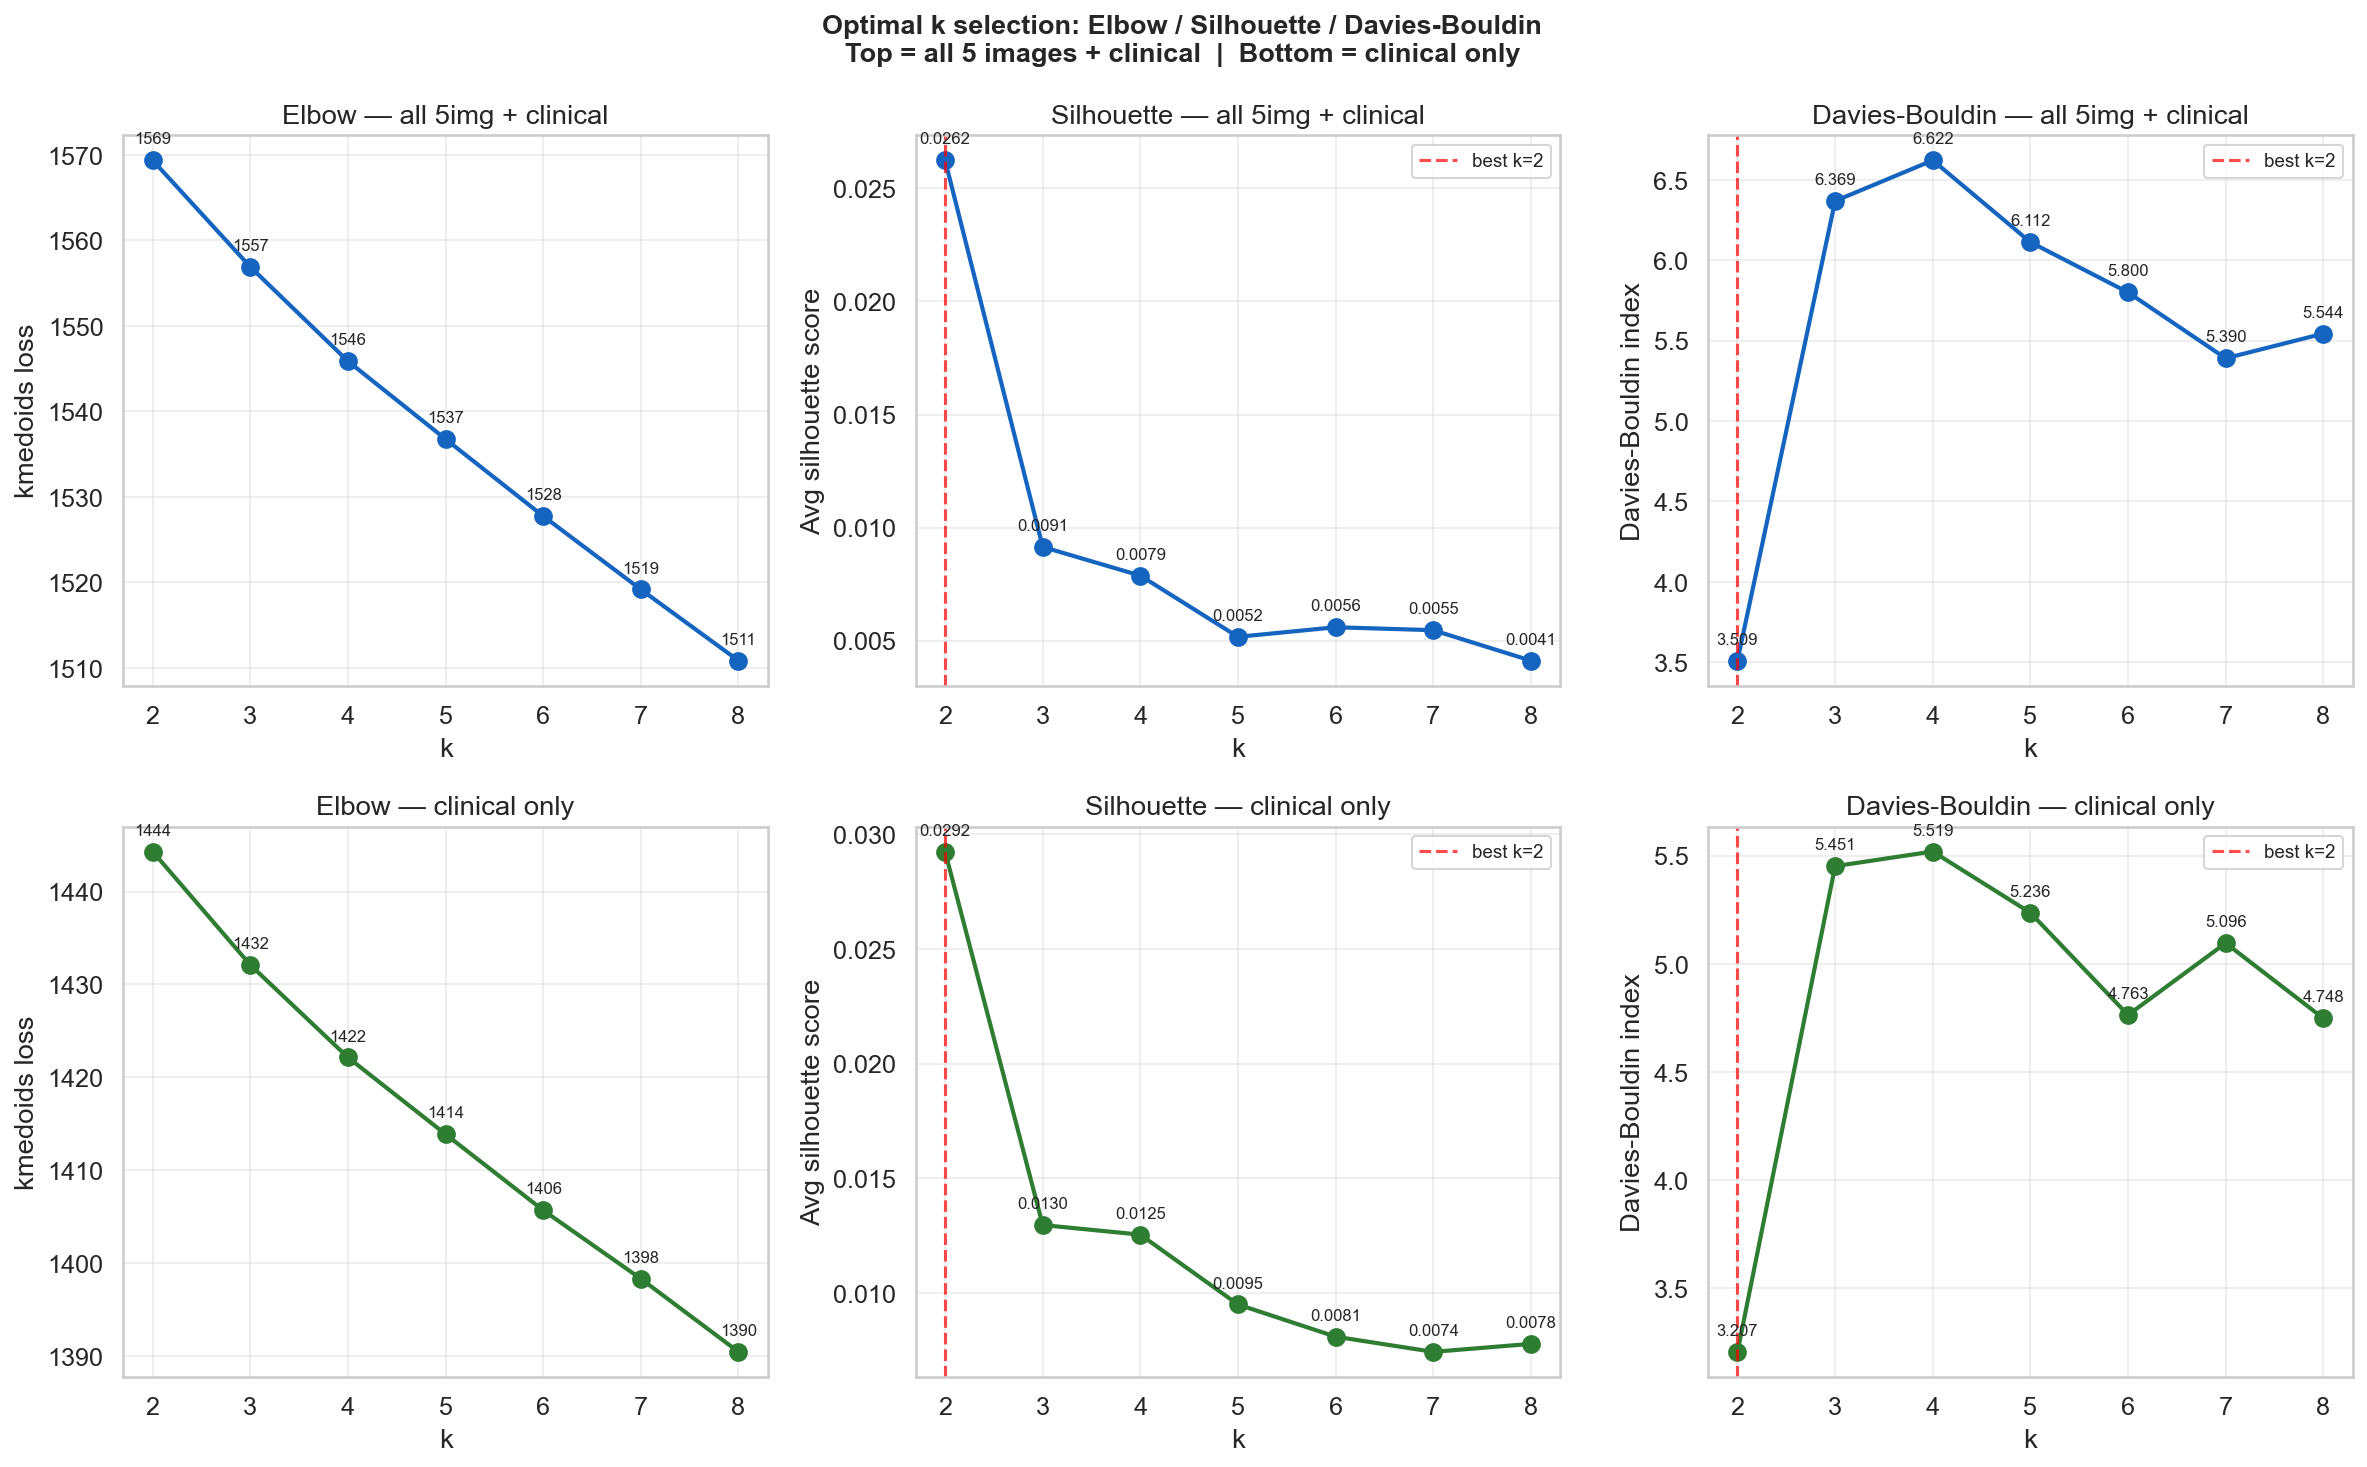
\includegraphics[width=\textwidth]{k_selection_criteria.png}
    \caption{k-selection criteria (k=2 to 8). Top row: all 5 images + clinical.
    Bottom row: clinical only. All three methods agree on $k=2$.}
    \label{fig:kselection}
\end{figure}

% ══════════════════════════════════════════════════════════════════════════════
\section{Experiment 1: All 5 Images + Clinical Data}

\subsection{Configuration}
Feature matrix: five image PCA blocks (110 components each) concatenated with 5 continuous
clinical features (p1) and 3 ordinal/nominal features (p3).
Shape: $216 \times 558$. Distance: RelMS.

\subsection{Evaluation}

\begin{table}[H]
\centering
\caption{Evaluation metrics — all 5 images + clinical.}
\begin{tabular}{ccccc}
\toprule
$k$ & \textbf{Silhouette} & \textbf{ARI vs CDR} & \textbf{NMI vs CDR} & Sizes \\
\midrule
2 & 0.0262 & 0.0283 & 0.0107 & 146 / 70 \\
3 & 0.0091 & 0.0176 & 0.0188 & 65 / 56 / 95 \\
\bottomrule
\end{tabular}
\end{table}

\subsection{Cluster Profiles}

\textbf{$k=2$} — The dominant split is by sex and brain volume (eTIV):

\begin{table}[H]
\centering
\caption{Cluster profiles — all 5 images + clinical, $k=2$.}
\begin{tabular}{lcc}
\toprule
\textbf{Feature} & \textbf{C0 ($n=146$)} & \textbf{C1 ($n=70$)} \\
\midrule
\% Female & \textbf{88.4\%} & 22.9\% \\
Age & $72.6 \pm 11.6$ & $72.1 \pm 13.8$ \\
MMSE & $27.4 \pm 3.5$ & $27.2 \pm 3.4$ \\
eTIV (mm$^3$) & $1375 \pm 93$ & $\mathbf{1633 \pm 128}$ \\
nWBV & $0.76 \pm 0.05$ & $0.74 \pm 0.05$ \\
Education & $2.95 \pm 1.22$ & $3.81 \pm 1.38$ \\
SES & $2.69 \pm 1.03$ & $2.07 \pm 1.20$ \\
\midrule
CDR=0 & 65.1\% & 54.3\% \\
CDR=0.5 & 22.6\% & 34.3\% \\
CDR=1 & 11.6\% & 10.0\% \\
CDR=2 & 0.7\% & 1.4\% \\
\bottomrule
\end{tabular}
\end{table}

\textbf{$k=3$} — The split refines into three groups primarily by sex, eTIV, and education/SES:

\begin{table}[H]
\centering
\caption{Cluster profiles — all 5 images + clinical, $k=3$.}
\begin{tabular}{lccc}
\toprule
\textbf{Feature} & \textbf{C0 ($n=65$)} & \textbf{C1 ($n=56$)} & \textbf{C2 ($n=95$)} \\
\midrule
\% Female & 76.9\% & 23.2\% & \textbf{86.3\%} \\
Age & $71.3 \pm 11.7$ & $72.4 \pm 13.5$ & $73.2 \pm 12.1$ \\
MMSE & $26.8 \pm 3.8$ & $27.6 \pm 3.0$ & $27.5 \pm 3.4$ \\
eTIV & $1430 \pm 96$ & $\mathbf{1661 \pm 123}$ & $1359 \pm 95$ \\
Education & $2.28 \pm 1.10$ & $\mathbf{4.18 \pm 1.15}$ & $3.33 \pm 1.14$ \\
SES & $3.29 \pm 1.06$ & $\mathbf{1.71 \pm 0.95}$ & $2.40 \pm 0.88$ \\
\midrule
CDR=0 & 56.9\% & 57.1\% & 67.4\% \\
CDR=0.5 & 23.1\% & 32.1\% & 25.3\% \\
CDR=1 & 18.5\% & 10.7\% & 6.3\% \\
CDR=2 & 1.5\% & 0.0\% & 1.1\% \\
\bottomrule
\end{tabular}
\end{table}

\subsection{Visualisations}

\begin{figure}[H]
    \centering
    \begin{subfigure}[b]{\textwidth}
        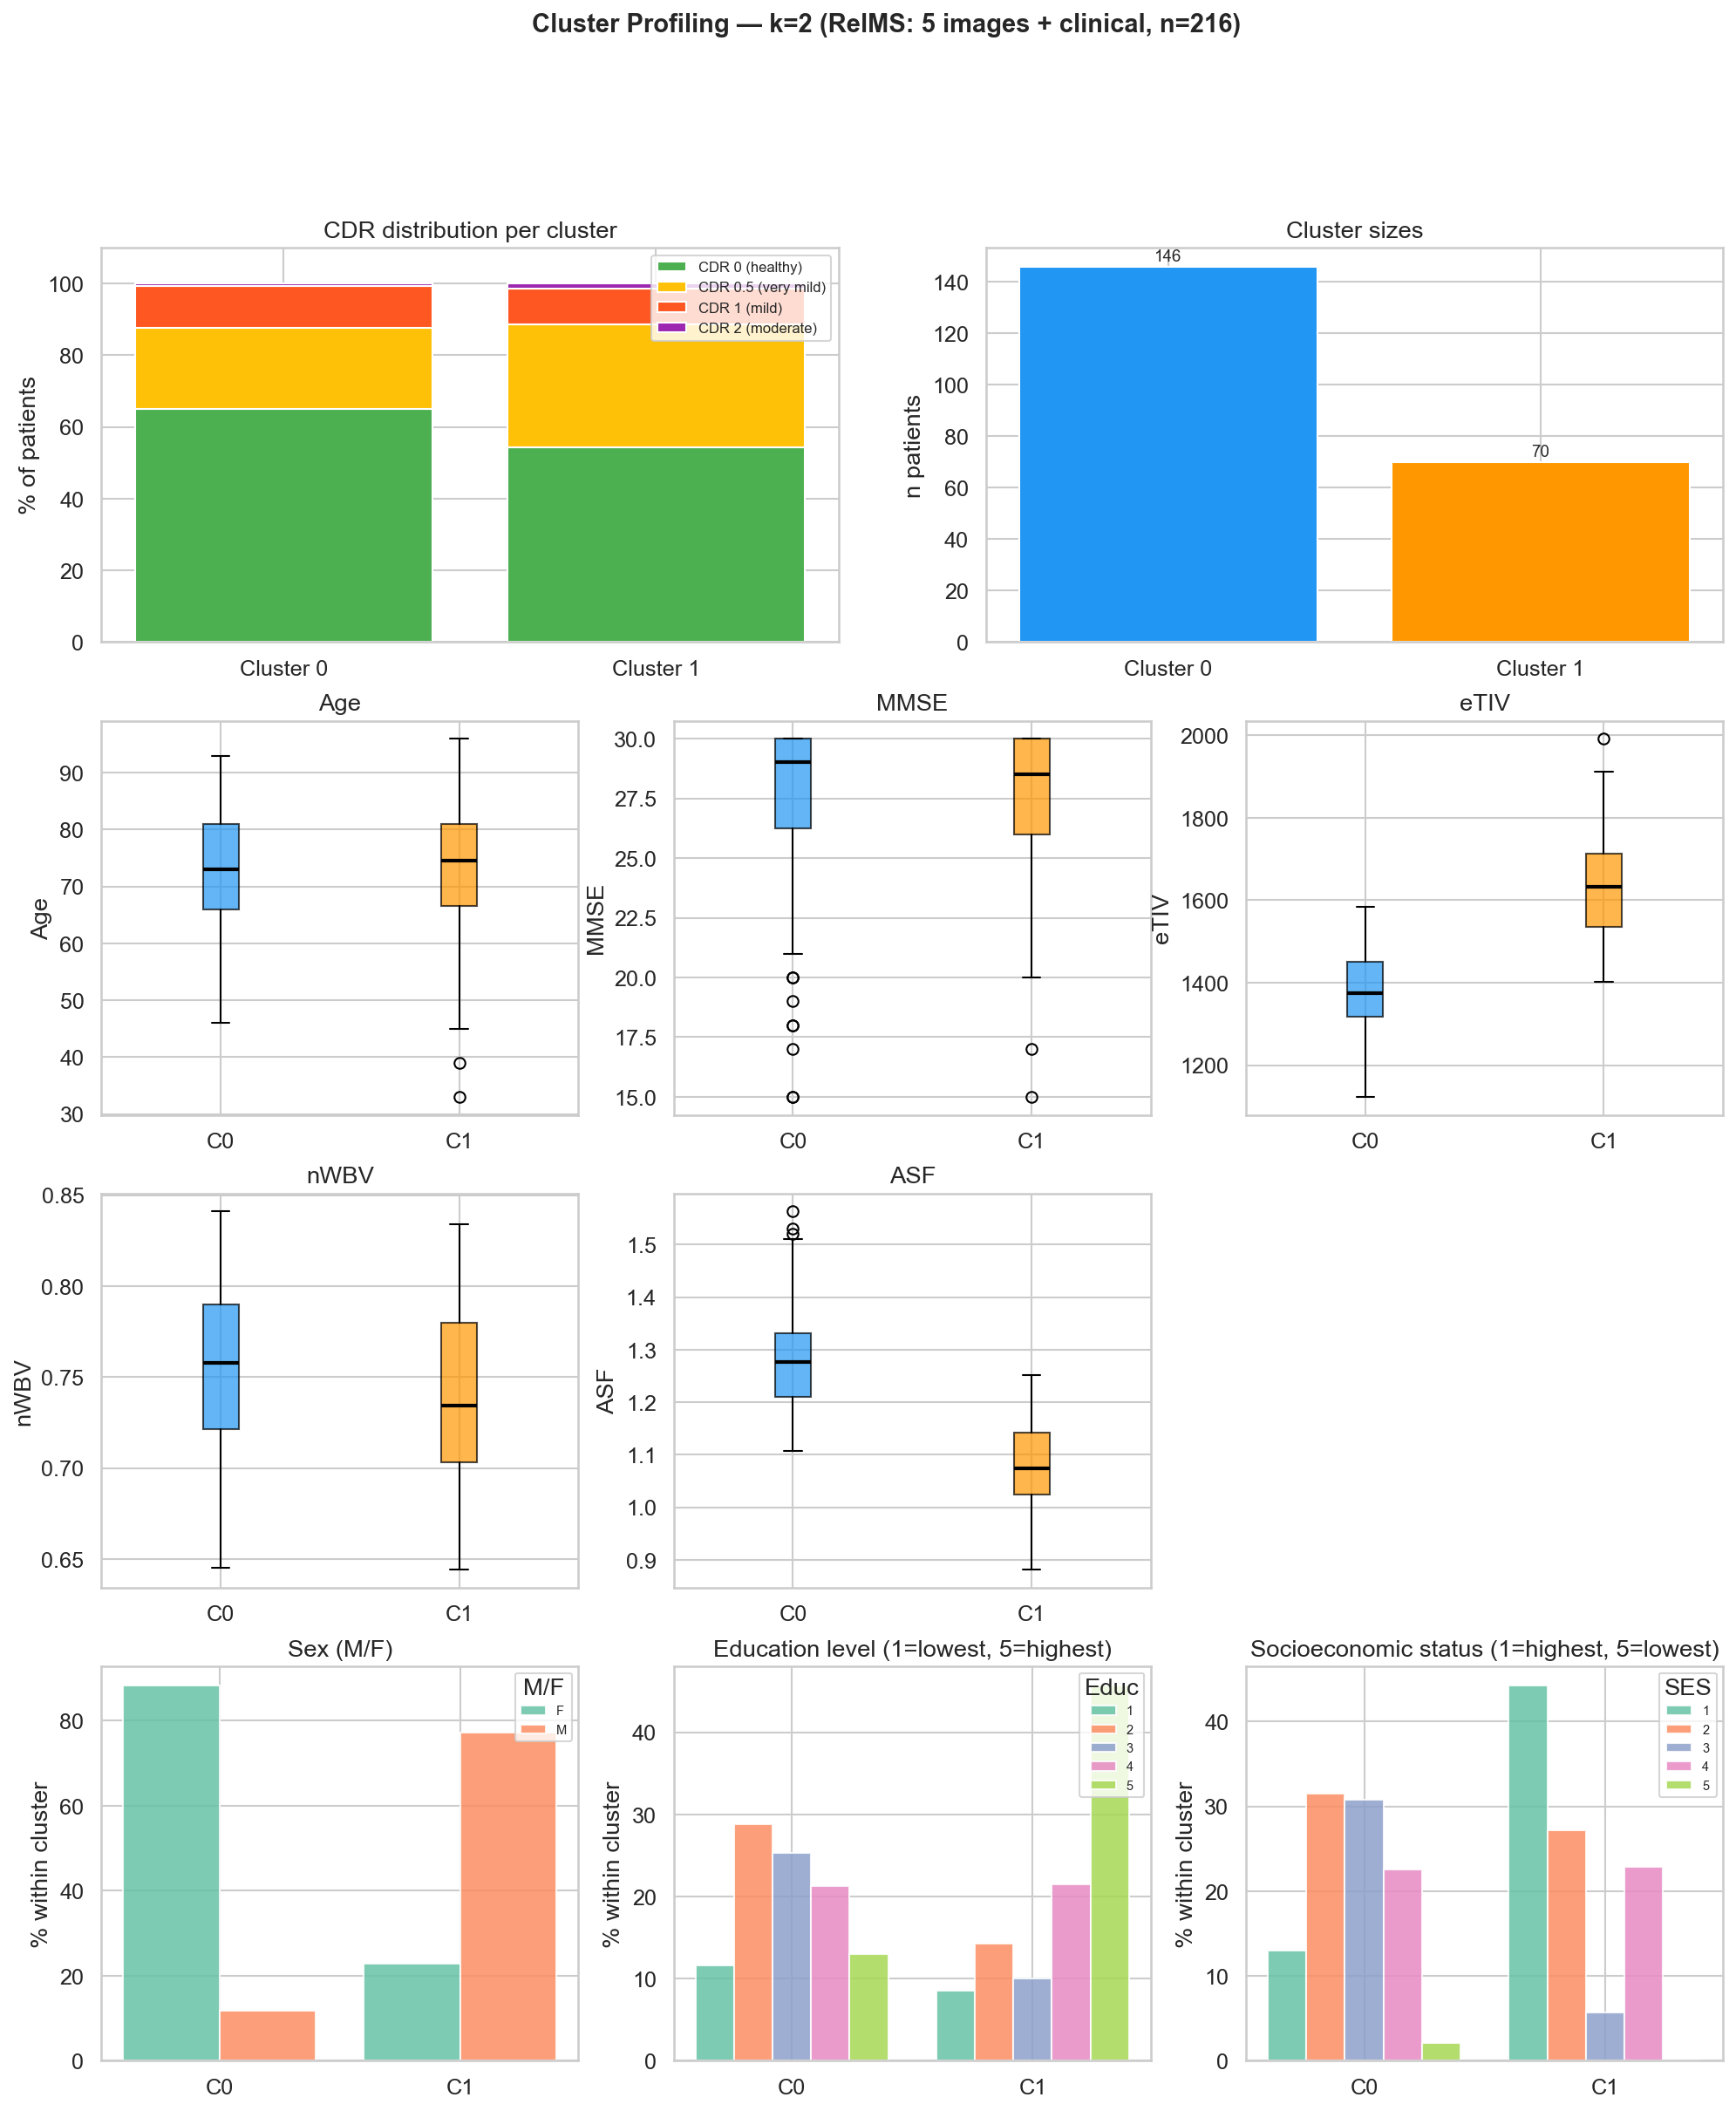
\includegraphics[width=\textwidth,height=0.42\textheight,keepaspectratio]{cluster_profile_k2.png}
        \caption{$k=2$}
    \end{subfigure}

    \begin{subfigure}[b]{\textwidth}
        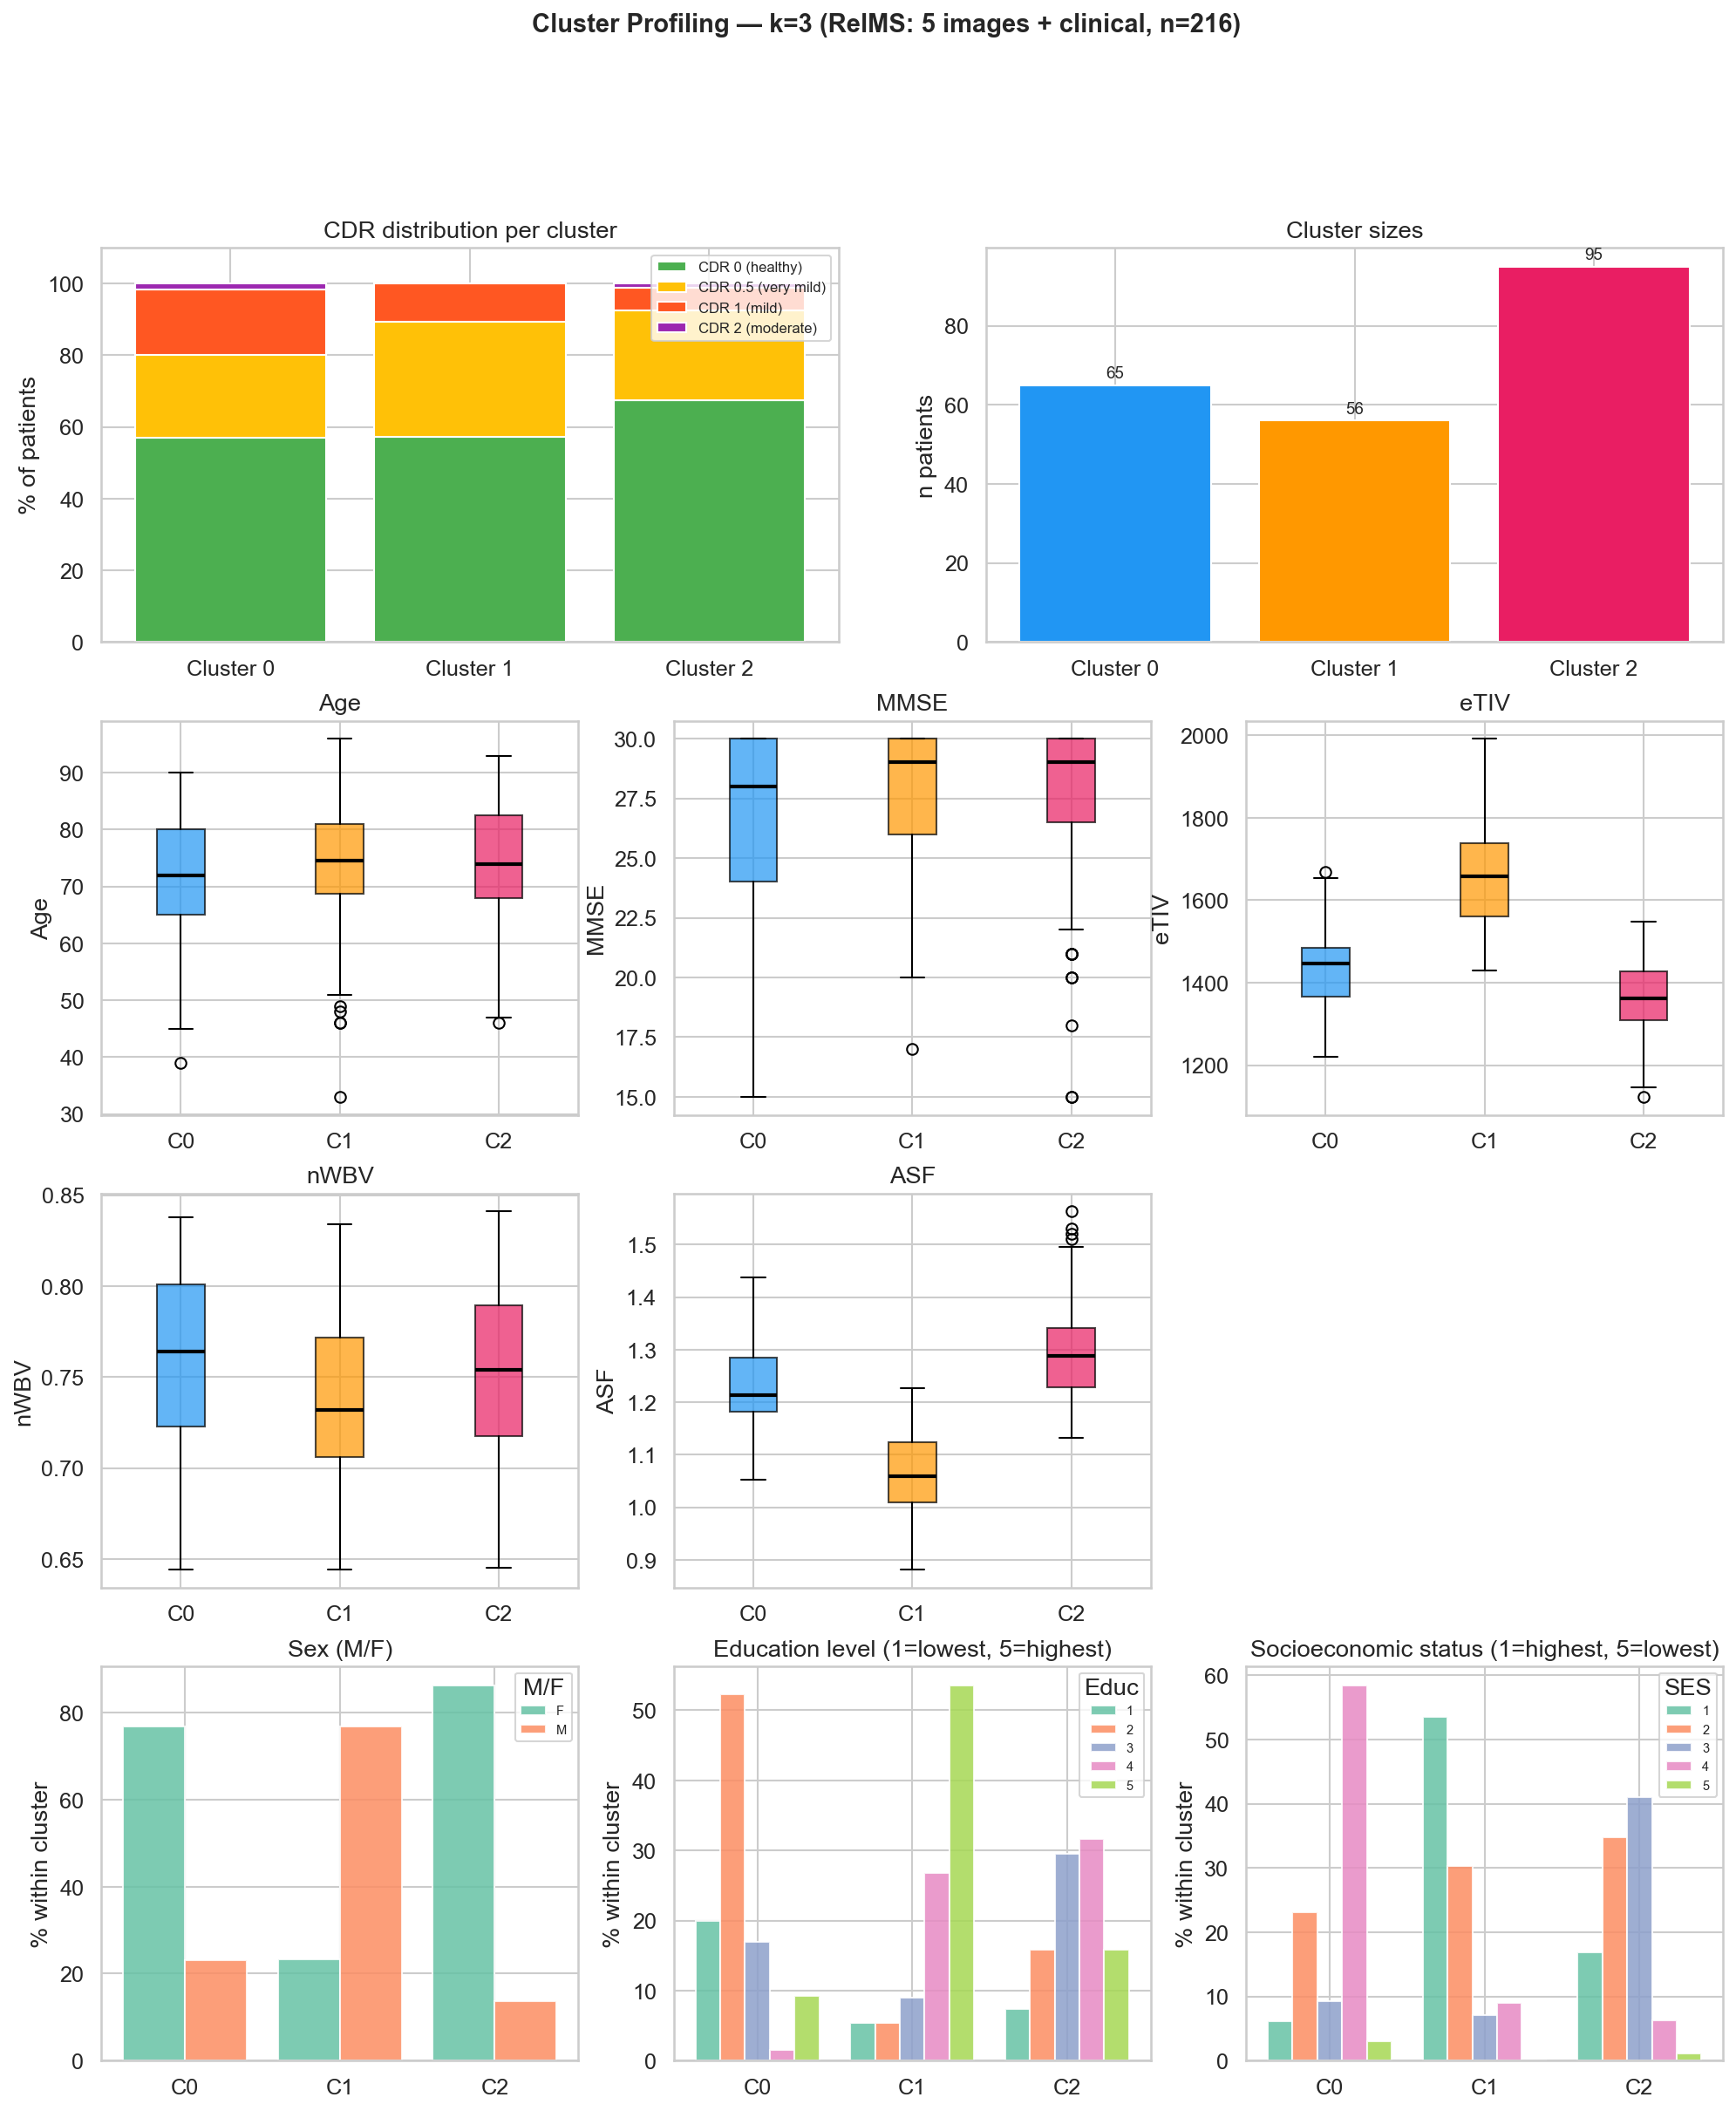
\includegraphics[width=\textwidth,height=0.42\textheight,keepaspectratio]{cluster_profile_k3.png}
        \caption{$k=3$}
    \end{subfigure}
    \caption{Cluster profiling — all 5 images + clinical. CDR distribution (top-left),
    cluster sizes (top-right), and boxplots for key clinical features.}
    \label{fig:full_profiles}
\end{figure}

\begin{figure}[H]
    \centering
    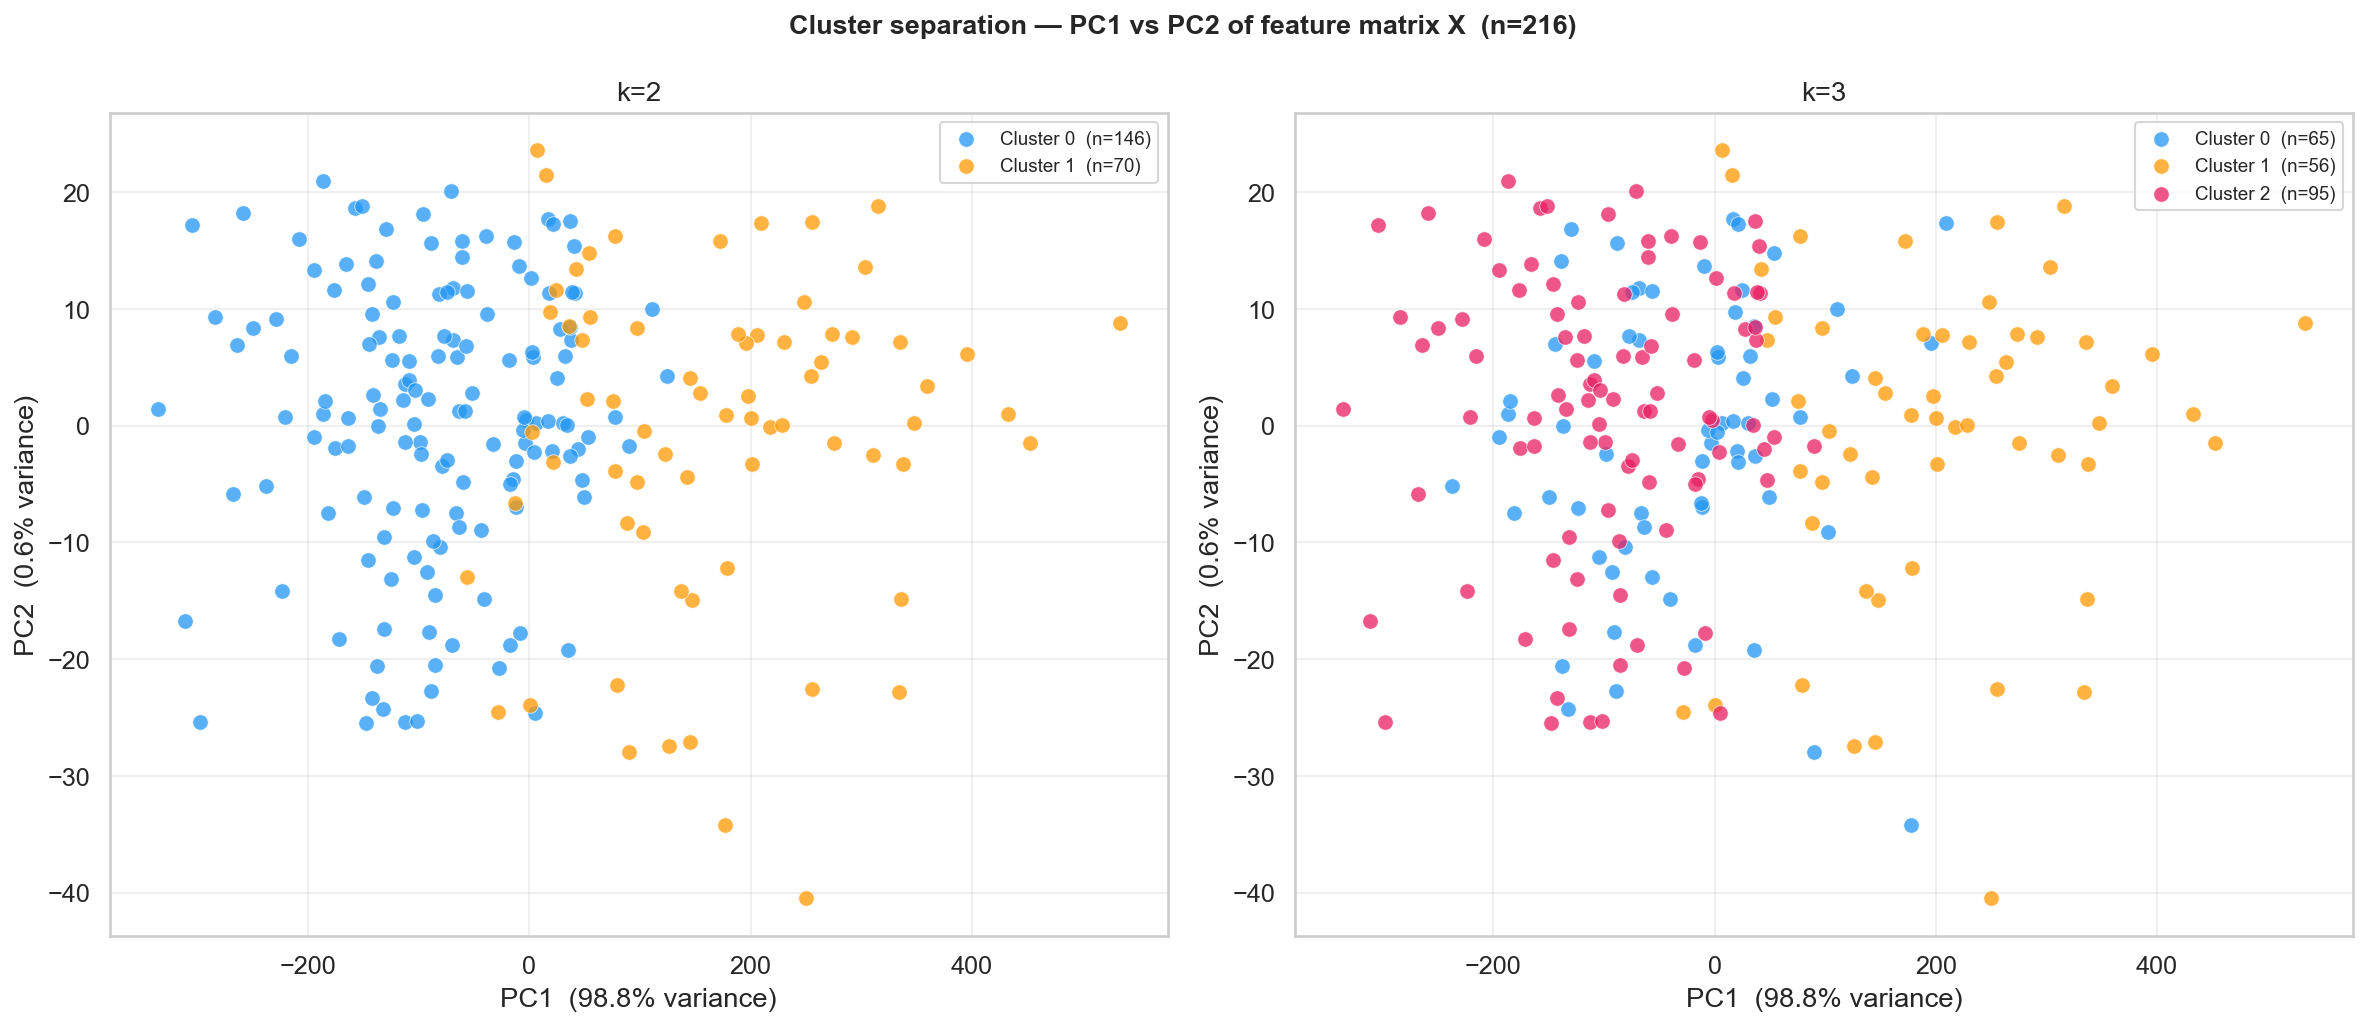
\includegraphics[width=0.95\textwidth]{cluster_pca_separation_n216.png}
    \caption{2D PCA scatter — all 5 images + clinical. PC1 explains 98.8\% of variance;
    the data lies essentially on a 1D axis.}
    \label{fig:full_pca2d}
\end{figure}

\begin{figure}[H]
    \centering
    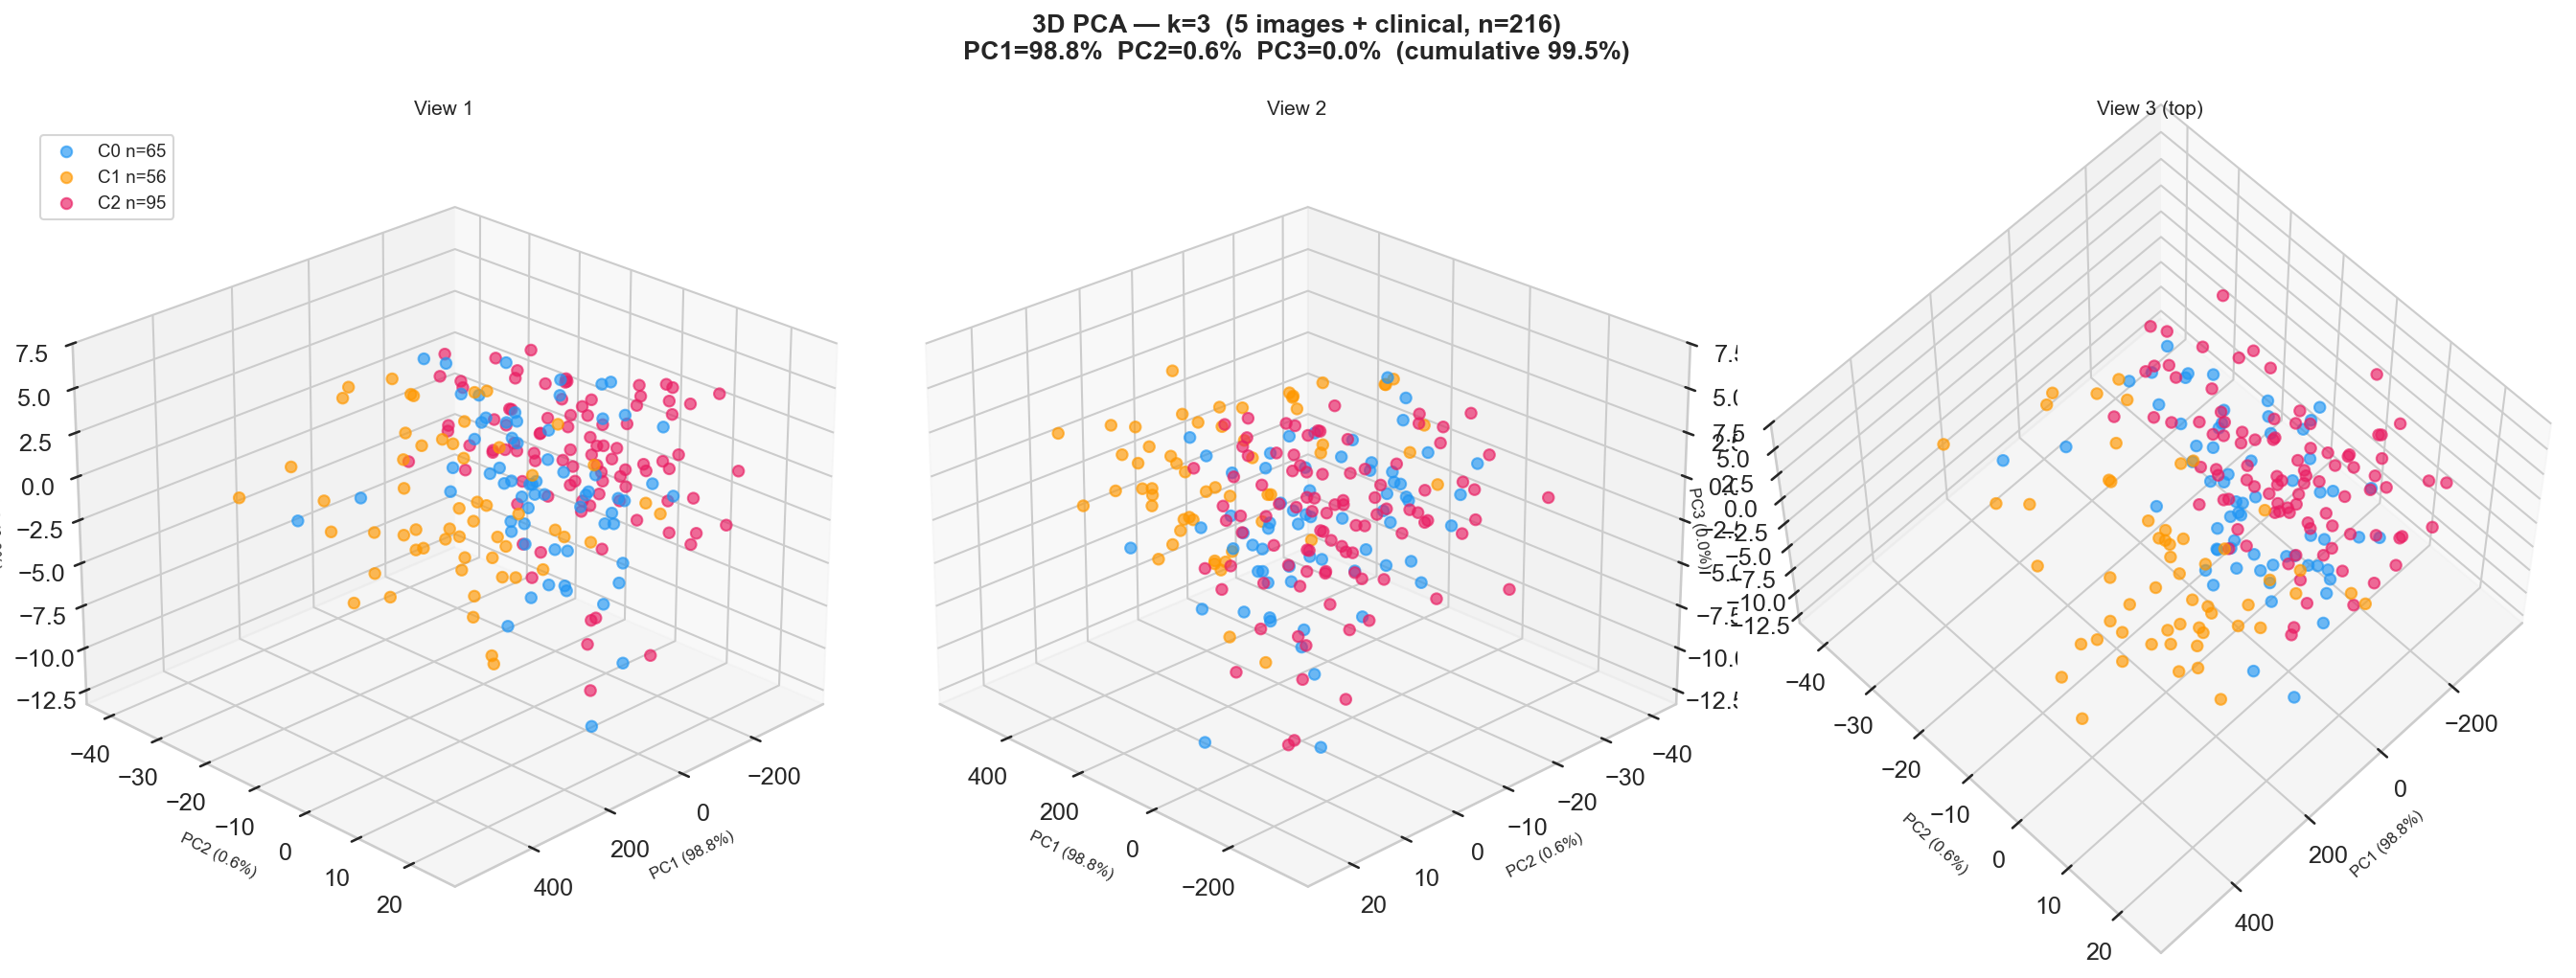
\includegraphics[width=\textwidth]{pca_3d_full_k3.png}
    \caption{3D PCA scatter — all 5 images + clinical, $k=3$ (three viewpoints).
    PC1=98.8\%, PC2=0.6\%, PC3=0.0\% (cumulative 99.5\%). The third dimension
    carries no information; clusters overlap heavily along the single dominant axis.}
    \label{fig:full_pca3d}
\end{figure}

\begin{figure}[H]
    \centering
    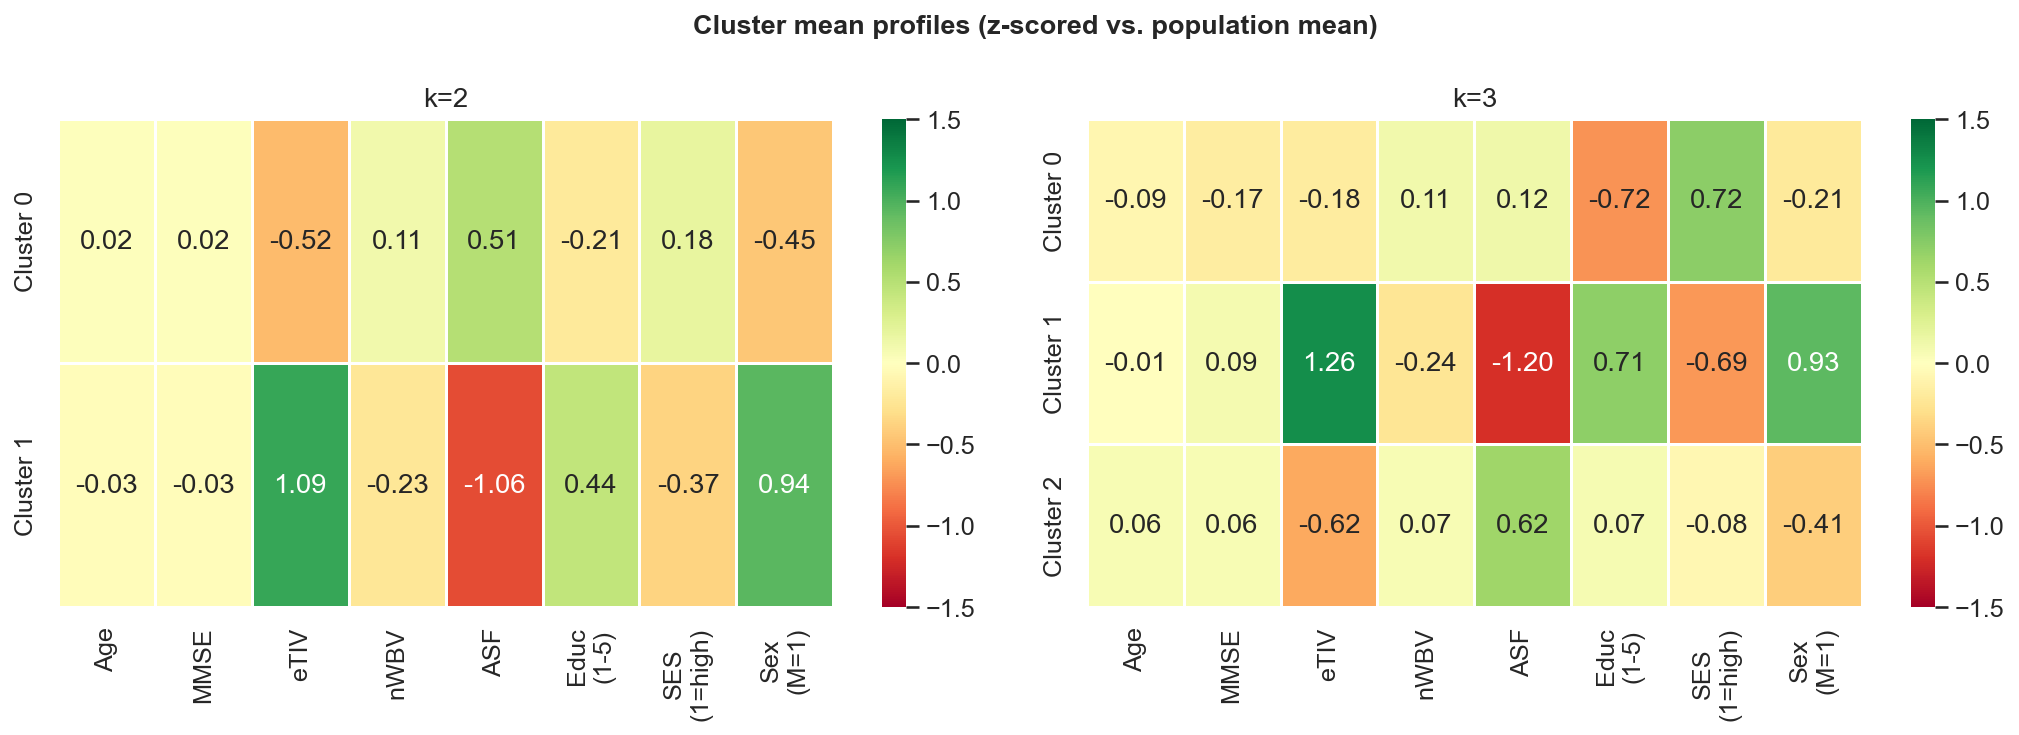
\includegraphics[width=0.9\textwidth]{cluster_profile_heatmap.png}
    \caption{Cluster mean heatmap (z-scored). Each cell shows how a cluster's mean
    deviates from the population mean. eTIV and sex (MF) are the strongest differentiators.}
    \label{fig:heatmap}
\end{figure}

% ══════════════════════════════════════════════════════════════════════════════
\section{Experiment 2: Clinical Data Only}

\subsection{Configuration}
Feature matrix: 5 continuous clinical features (p1) + 3 ordinal/nominal features (p3).
Shape: $216 \times 8$. Distance: RelMS.

\subsection{Evaluation}

\begin{table}[H]
\centering
\caption{Evaluation metrics — clinical only.}
\begin{tabular}{ccccc}
\toprule
$k$ & \textbf{Silhouette} & \textbf{ARI vs CDR} & Sizes \\
\midrule
2 & 0.0292 & 0.0245 & 147 / 69 \\
3 & 0.0130 & 0.0177 & 78 / 62 / 76 \\
\bottomrule
\end{tabular}
\end{table}

\subsection{Cluster Profiles}

\textbf{$k=2$} — Almost identical to the full experiment, confirming that clinical features
dominate the distance matrix:

\begin{table}[H]
\centering
\caption{Cluster profiles — clinical only, $k=2$.}
\begin{tabular}{lcc}
\toprule
\textbf{Feature} & \textbf{C0 ($n=147$)} & \textbf{C1 ($n=69$)} \\
\midrule
\% Female & \textbf{87.8\%} & 23.2\% \\
Age & $72.3 \pm 11.8$ & $72.8 \pm 13.5$ \\
MMSE & $27.3 \pm 3.6$ & $27.5 \pm 3.2$ \\
eTIV & $1377 \pm 95$ & $\mathbf{1633 \pm 131}$ \\
Education & $2.93 \pm 1.23$ & $3.88 \pm 1.32$ \\
SES & $2.73 \pm 1.03$ & $1.99 \pm 1.14$ \\
\midrule
CDR=0 & 64.6\% & 55.1\% \\
CDR=0.5 & 23.8\% & 31.9\% \\
CDR=1 & 10.9\% & 11.6\% \\
CDR=2 & 0.7\% & 1.4\% \\
\bottomrule
\end{tabular}
\end{table}

\textbf{$k=3$} — Three groups emerge defined by sex, brain size, and socioeconomic factors:

\begin{table}[H]
\centering
\caption{Cluster profiles — clinical only, $k=3$.}
\begin{tabular}{lccc}
\toprule
\textbf{Feature} & \textbf{C0 ($n=78$)} & \textbf{C1 ($n=62$)} & \textbf{C2 ($n=76$)} \\
\midrule
\% Female & \textbf{91.0\%} & 24.2\% & 77.6\% \\
Age & $70.1 \pm 13.1$ & $72.2 \pm 13.9$ & $75.0 \pm 9.4$ \\
MMSE & $27.9 \pm 3.2$ & $27.6 \pm 2.9$ & $26.6 \pm 3.9$ \\
eTIV & $1354 \pm 96$ & $\mathbf{1649 \pm 125}$ & $1411 \pm 89$ \\
Education & $3.72 \pm 1.03$ & $\mathbf{4.06 \pm 1.20}$ & $2.05 \pm 0.78$ \\
SES & $2.08 \pm 0.75$ & $1.84 \pm 1.03$ & $\mathbf{3.45 \pm 0.84}$ \\
\midrule
CDR=0 & 74.4\% & 56.5\% & 52.6\% \\
CDR=0.5 & 19.2\% & 32.3\% & 28.9\% \\
CDR=1 & 6.4\% & 11.3\% & 15.8\% \\
CDR=2 & 0.0\% & 0.0\% & 2.6\% \\
\bottomrule
\end{tabular}
\end{table}

\subsection{Visualisations}

\begin{figure}[H]
    \centering
    \begin{subfigure}[b]{\textwidth}
        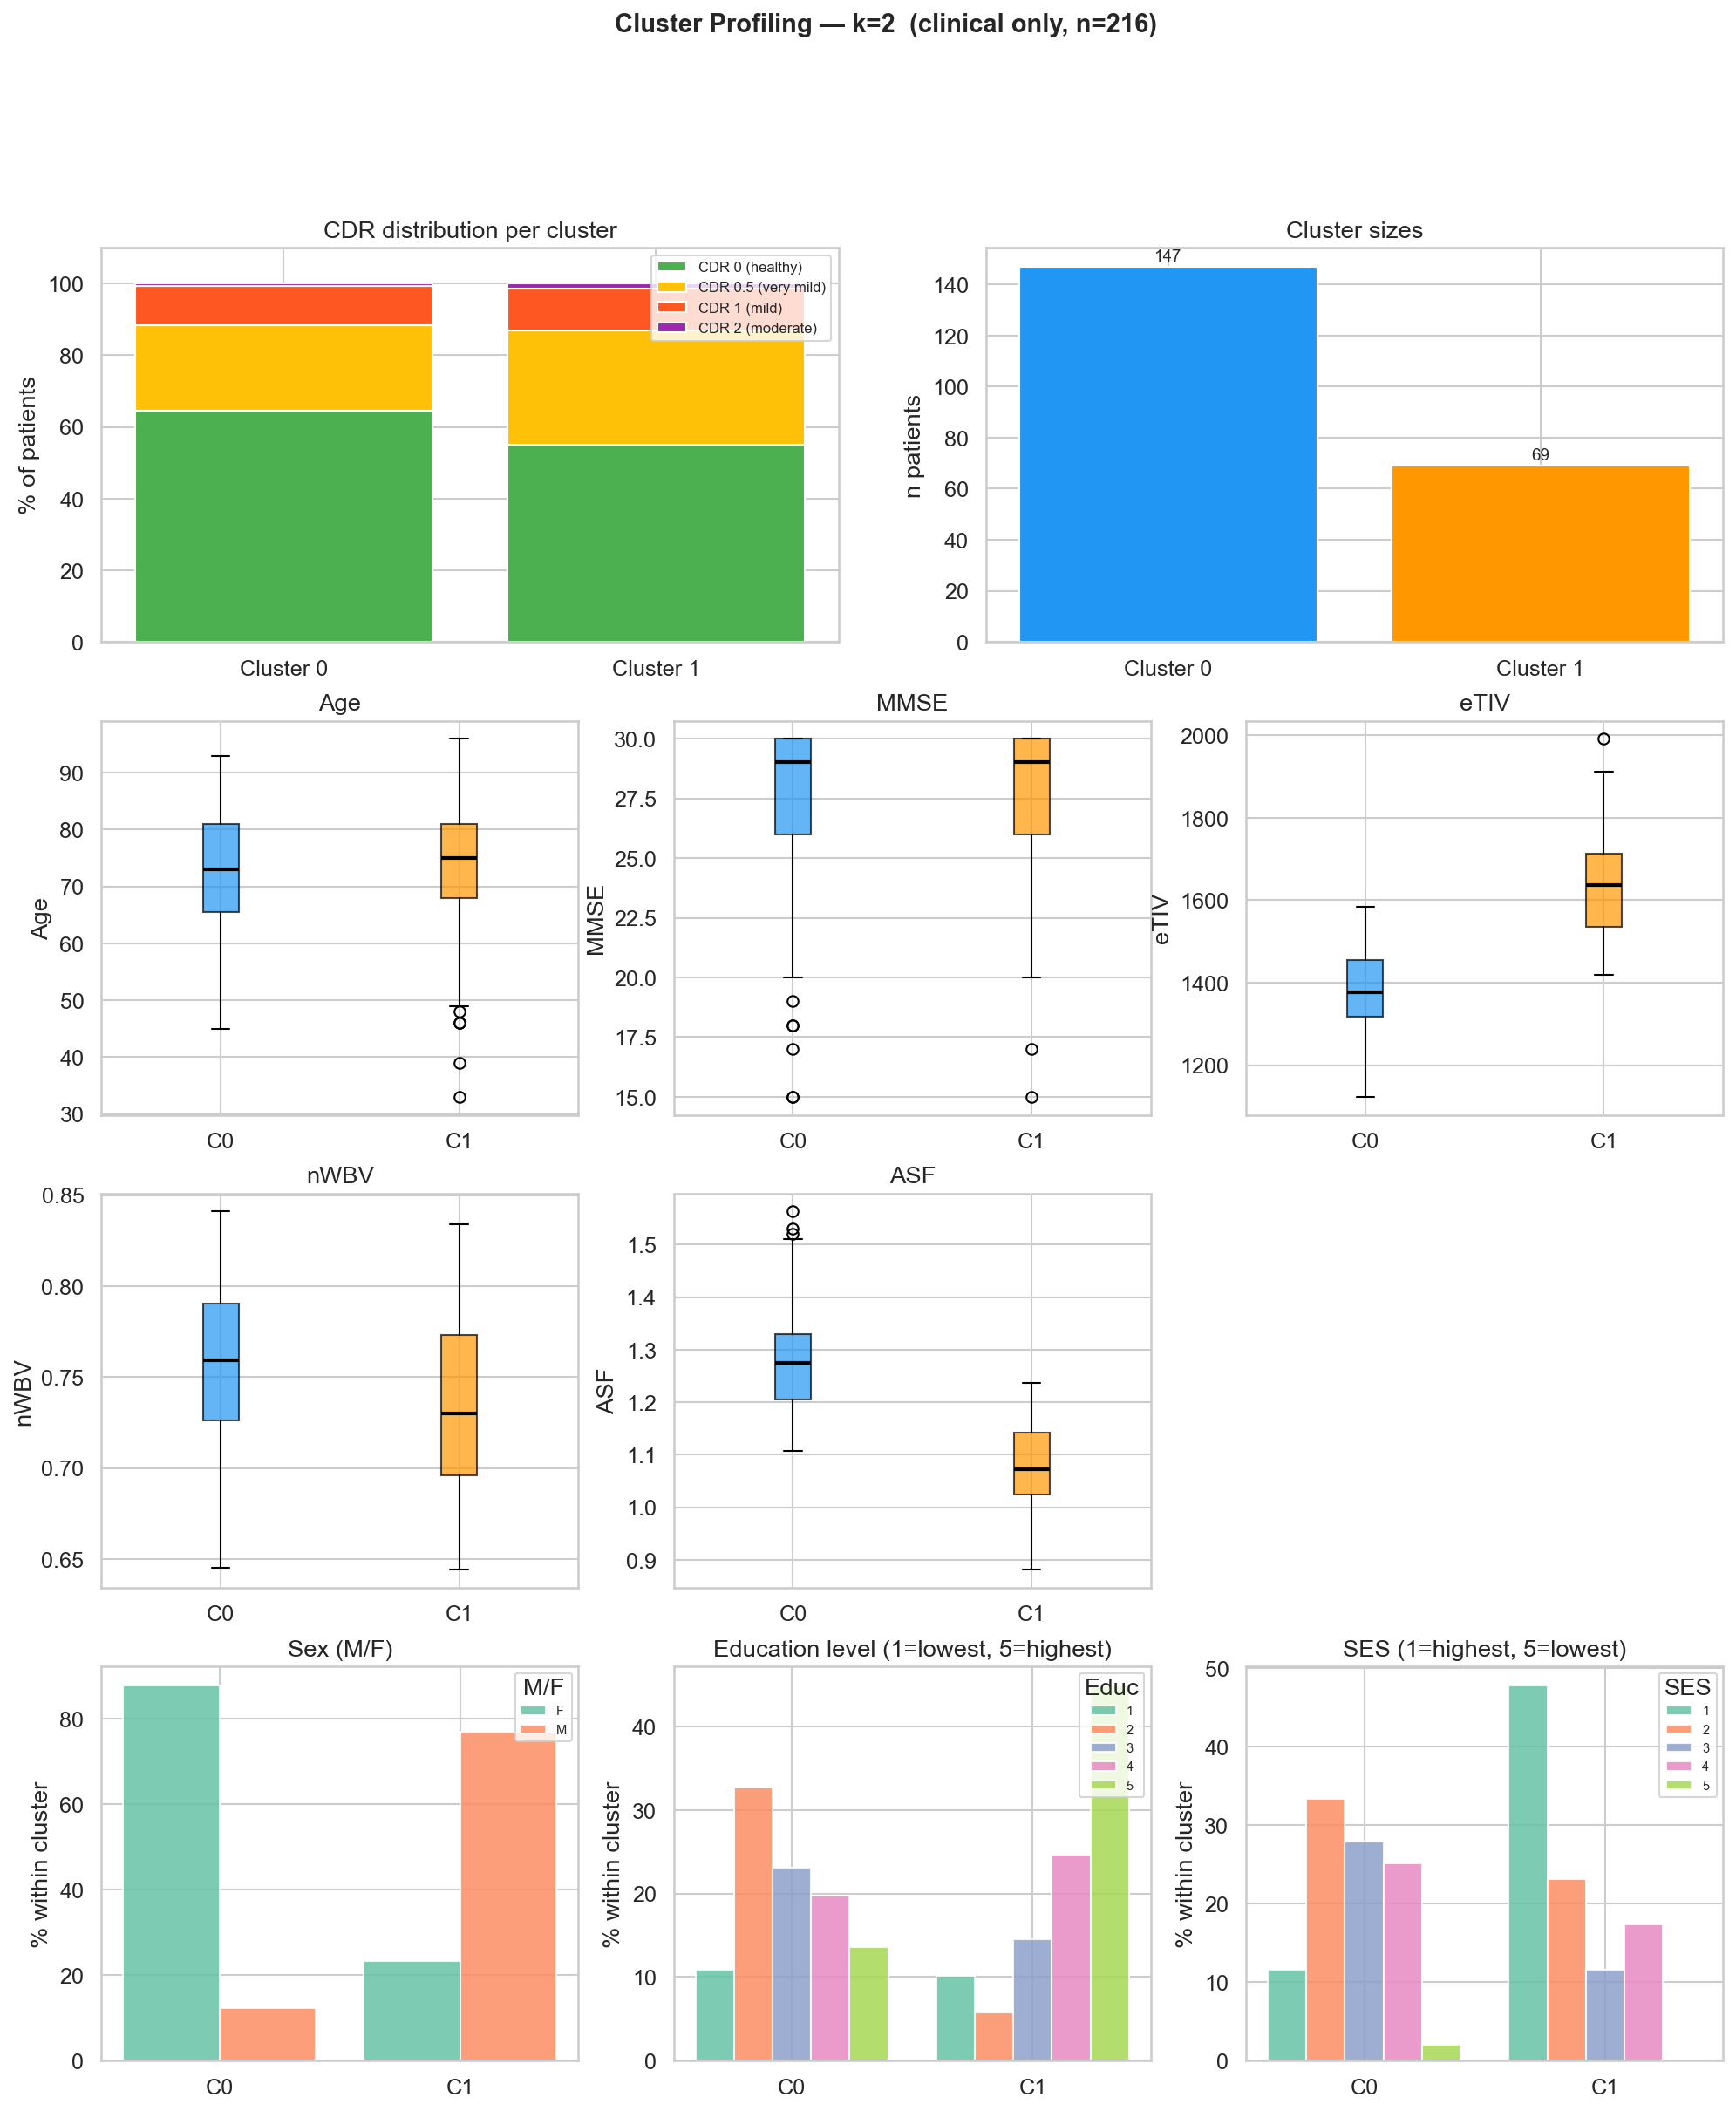
\includegraphics[width=\textwidth,height=0.42\textheight,keepaspectratio]{clinical_only_profile_k2.png}
        \caption{$k=2$}
    \end{subfigure}

    \begin{subfigure}[b]{\textwidth}
        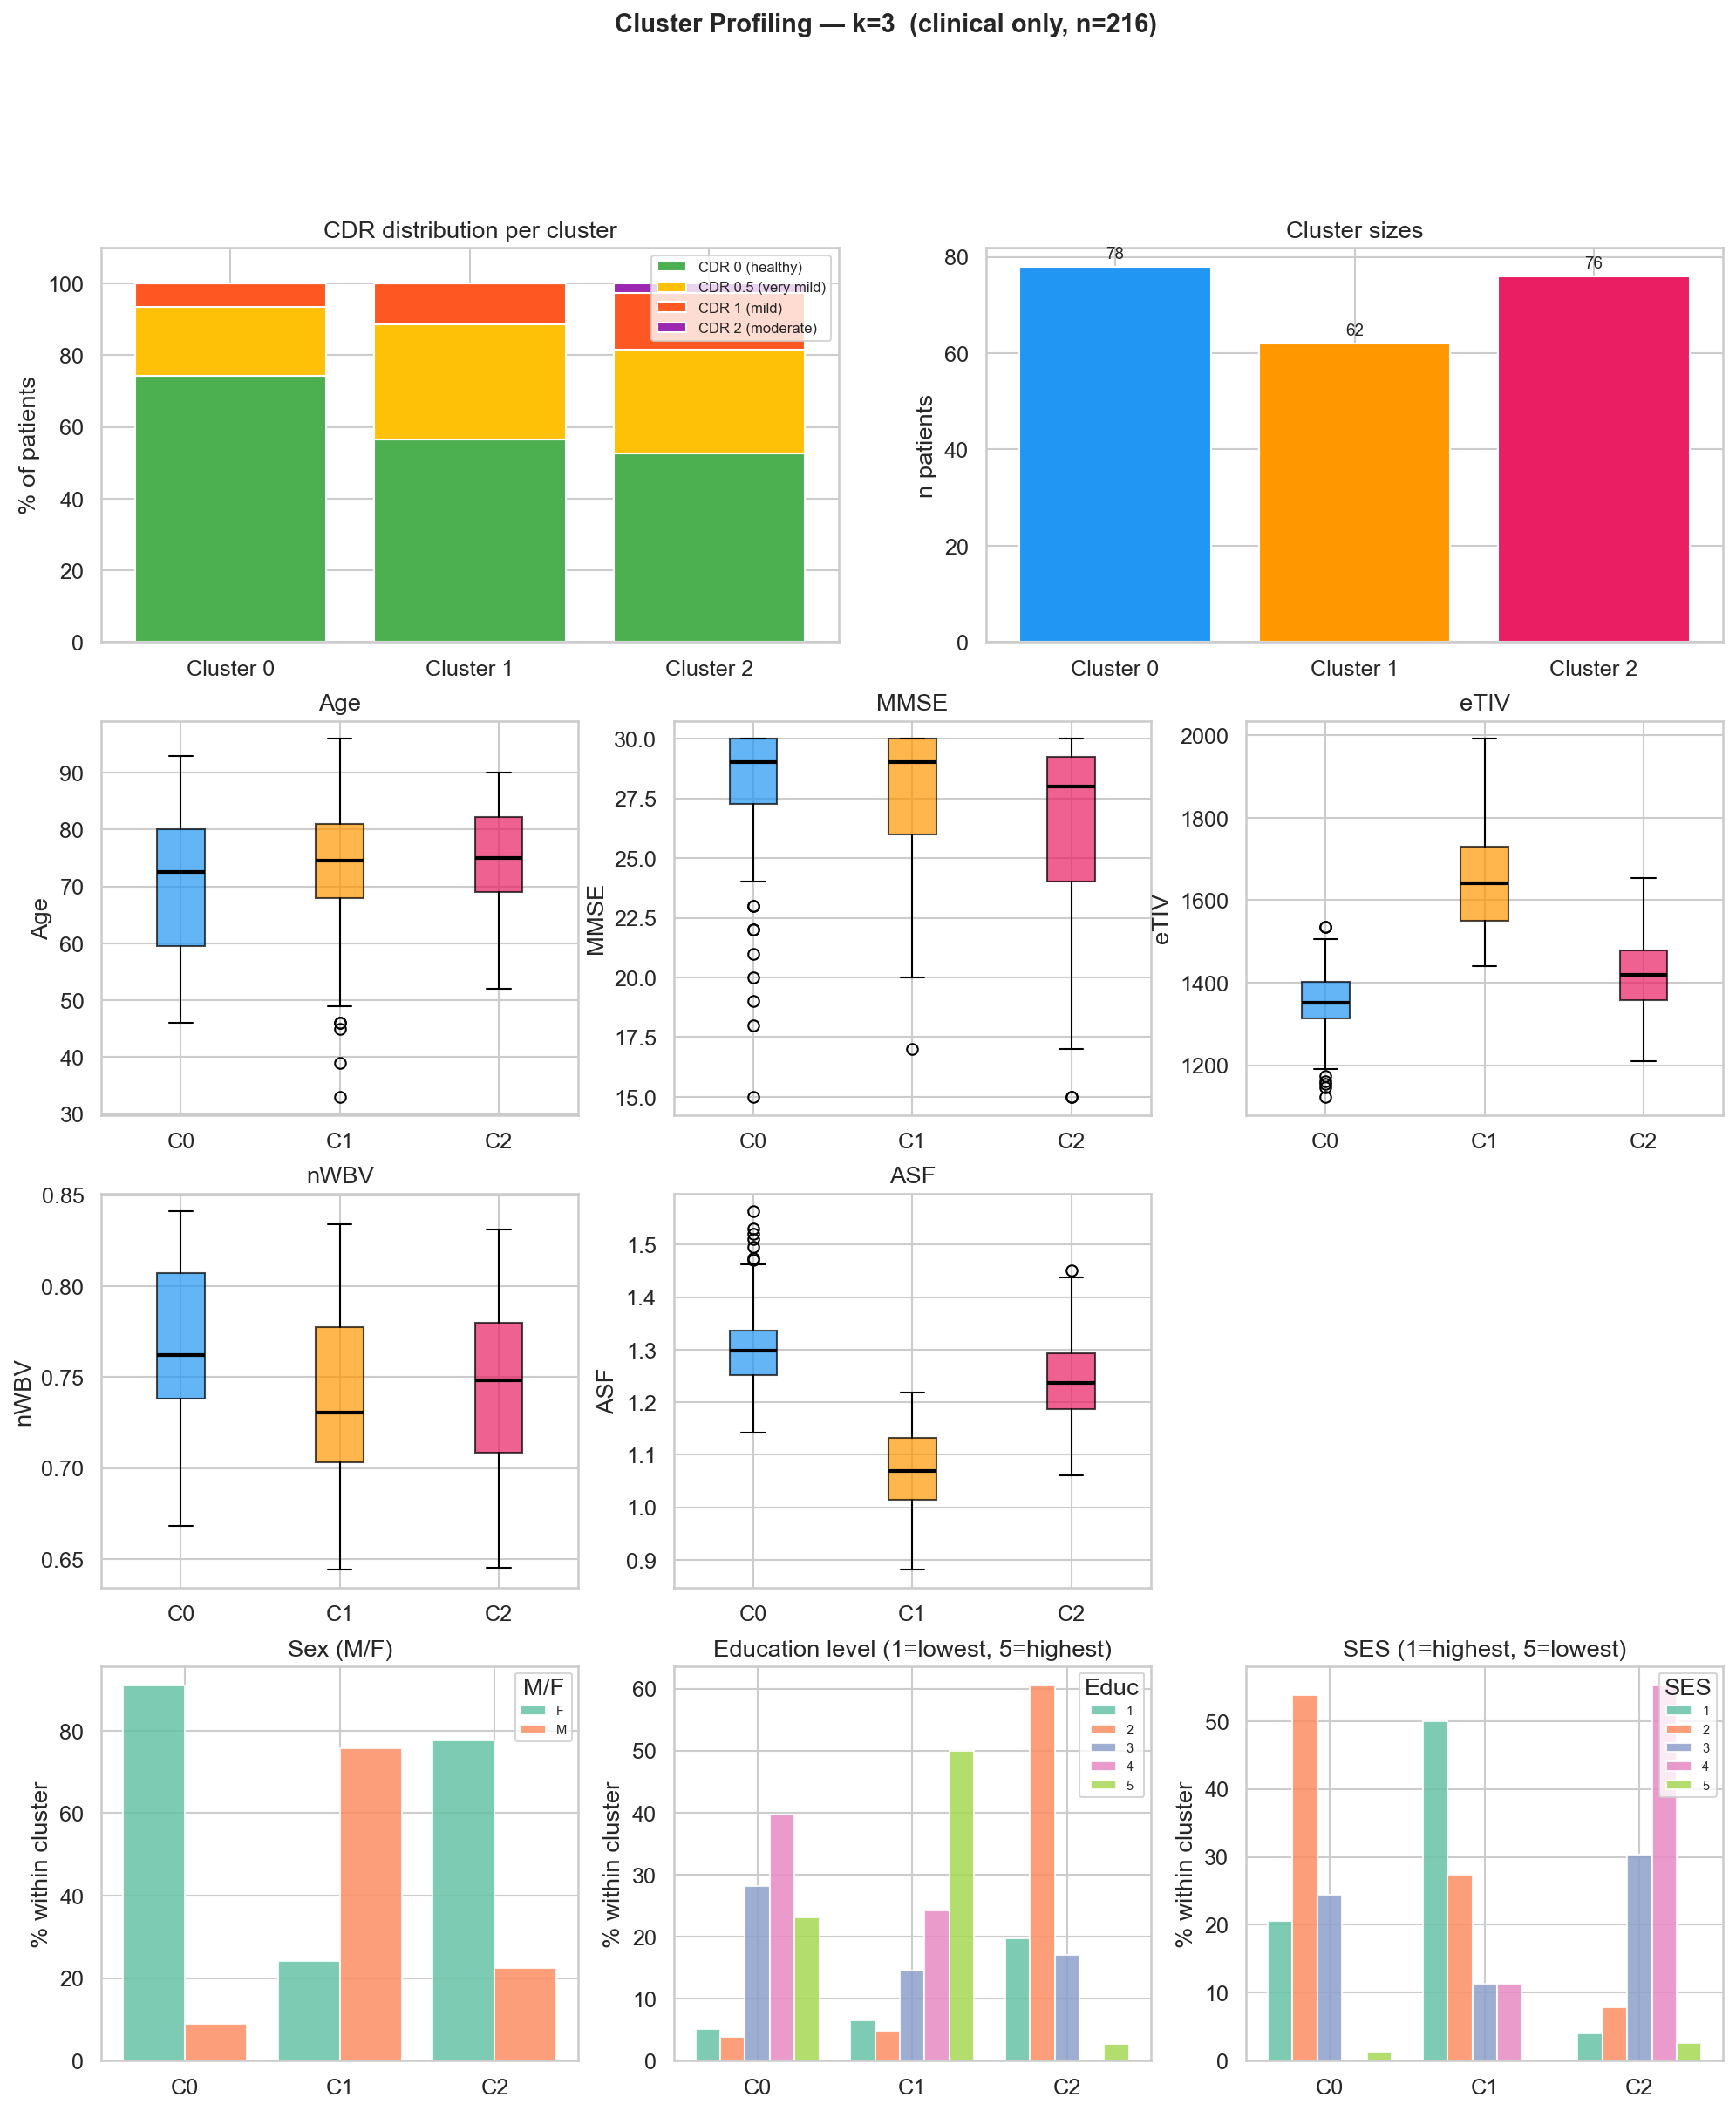
\includegraphics[width=\textwidth,height=0.42\textheight,keepaspectratio]{clinical_only_profile_k3.png}
        \caption{$k=3$}
    \end{subfigure}
    \caption{Cluster profiling — clinical only.}
    \label{fig:clin_profiles}
\end{figure}

\begin{figure}[H]
    \centering
    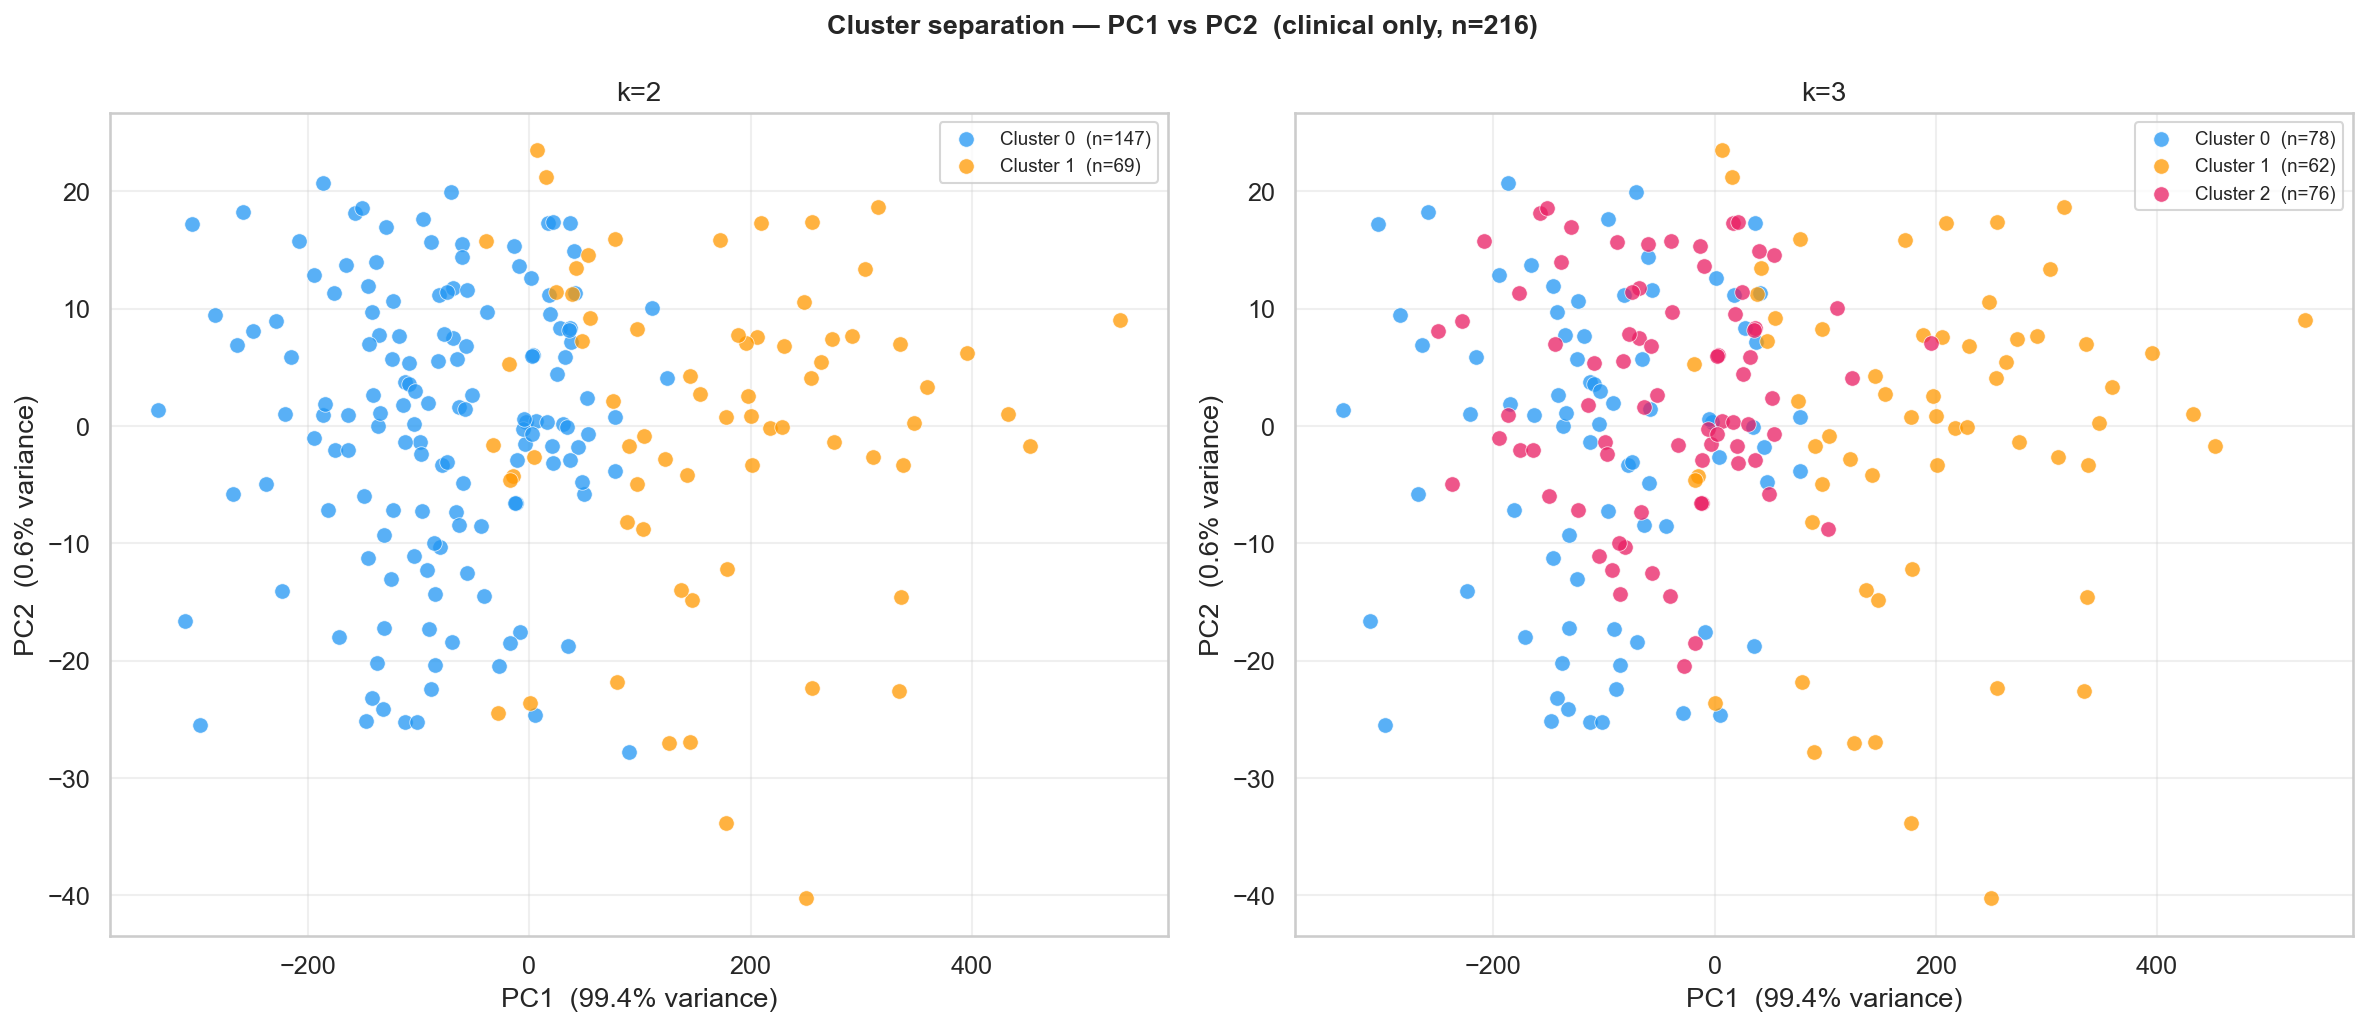
\includegraphics[width=0.95\textwidth]{clinical_only_pca_scatter.png}
    \caption{2D PCA scatter — clinical only. PC1 = 99.4\% of variance.}
    \label{fig:clin_pca2d}
\end{figure}

\begin{figure}[H]
    \centering
    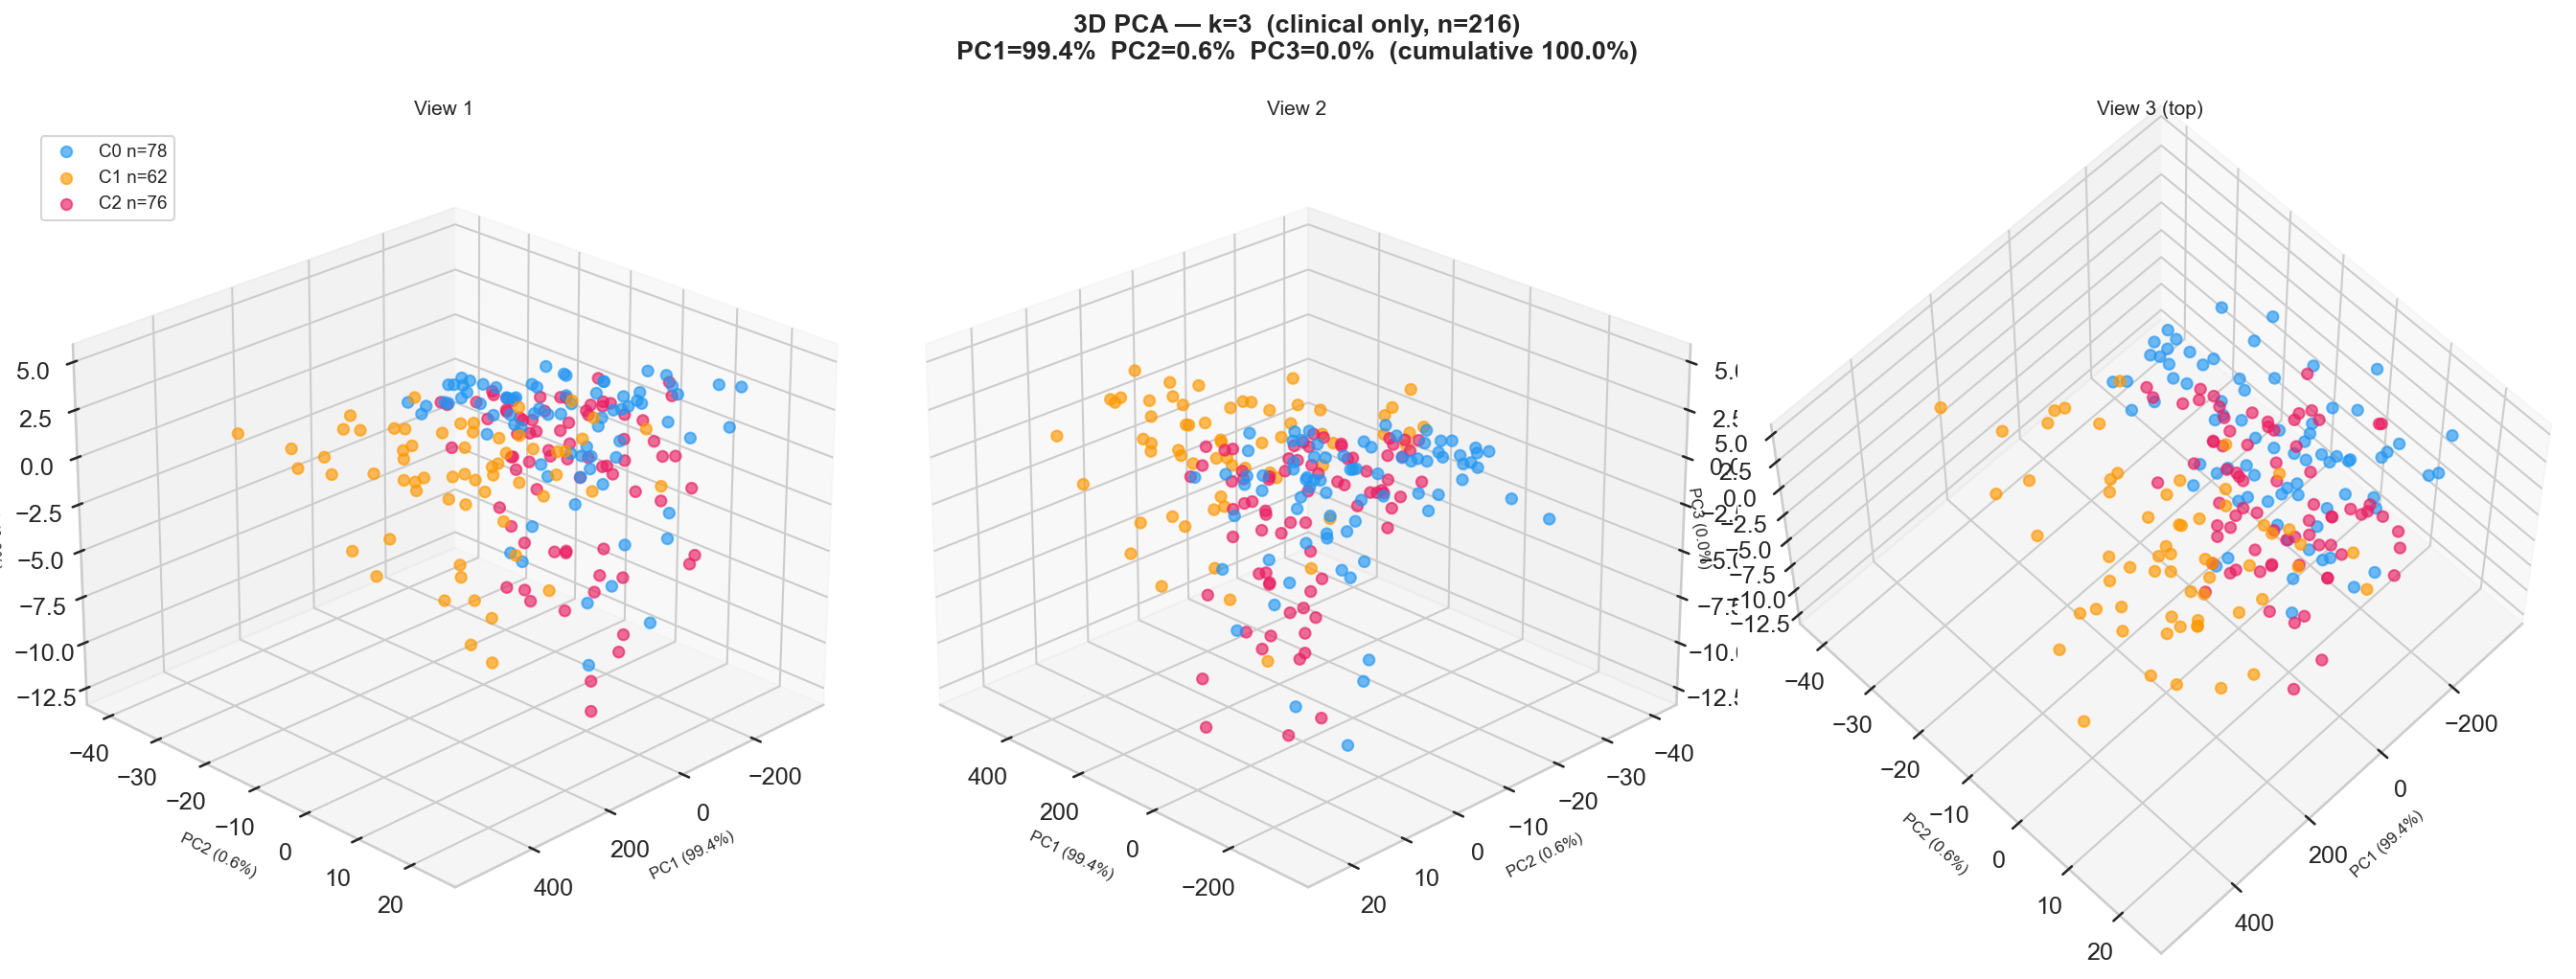
\includegraphics[width=\textwidth]{pca_3d_clinical_k3.png}
    \caption{3D PCA scatter — clinical only, $k=3$ (three viewpoints).
    PC1=99.4\%, PC2=0.6\%, PC3=0.0\%. The dataset is effectively 1-dimensional;
    no additional separation is visible in the third dimension.}
    \label{fig:clin_pca3d}
\end{figure}

% ══════════════════════════════════════════════════════════════════════════════
\section{Experiment 3: Images Only (Baseline)}

\subsection{Configuration}
Feature matrix: five image PCA blocks concatenated (no clinical features).
Shape: $216 \times 550$. Distance: Euclidean (all features are PCA components on
comparable scales; no mixed types).

\subsection{Evaluation}

\begin{table}[H]
\centering
\caption{Evaluation metrics — images only.}
\begin{tabular}{cccc}
\toprule
$k$ & \textbf{Silhouette} & \textbf{ARI vs CDR} & Sizes \\
\midrule
2 & 0.0510 & $-$0.0040 & 81 / 135 \\
3 & 0.0376 & $-$0.0205 & 35 / 100 / 81 \\
\bottomrule
\end{tabular}
\end{table}

The ARI vs CDR is negative for both $k$ values: image-only clusters are
\emph{worse than random} at predicting CDR category. The slightly higher silhouette
(compared to clinical experiments) reflects more uniform Euclidean distances,
not meaningful cluster quality.

\subsection{Image PCA Structure}

Unlike clinical data, image variance is distributed across many components:
\begin{itemize}[noitemsep]
    \item PC1: 8.18\% \quad PC2: 4.80\% \quad PC3: 4.24\% \quad PC4: 3.09\% \quad PC5: 2.82\%
    \item Cumulative top 5: 23.1\%
\end{itemize}

The first 5 components of the combined image space explain only 23\% of variance,
compared to 99\%+ in the clinical space. Image data is far higher-dimensional.

\subsection{Cluster Profiles — PC1–PC5}

Since clinical features were not used, clusters are profiled by their image PCA components.
CDR and M/F are shown as external labels only.

\begin{table}[H]
\centering
\caption{Image PCA components per cluster — images only, $k=2$.
CDR and M/F are external labels not used in clustering.}
\begin{tabular}{lcc}
\toprule
\textbf{Component} & \textbf{C0 ($n=81$)} & \textbf{C1 ($n=135$)} \\
\midrule
PC1 (8.18\%) & $+3.44 \pm 1.49$ & $-2.06 \pm 2.46$ \\
PC2 (4.80\%) & $+0.83 \pm 2.75$ & $-0.50 \pm 2.41$ \\
PC3 (4.24\%) & $-0.60 \pm 1.98$ & $+0.36 \pm 2.65$ \\
PC4 (3.09\%) & $-0.21 \pm 1.88$ & $+0.12 \pm 2.22$ \\
PC5 (2.82\%) & $+0.25 \pm 1.82$ & $-0.15 \pm 2.10$ \\
\midrule
CDR=0 (ext.) & 63.0\% & 60.7\% \\
\% Female (ext.) & 58.0\% & 72.6\% \\
\bottomrule
\end{tabular}
\end{table}

The split is almost entirely on PC1; PC2–PC5 differences are small relative to within-cluster
standard deviations. The CDR proportions are virtually identical between clusters.

\subsection{Visualisations}

\begin{figure}[H]
    \centering
    \begin{subfigure}[b]{\textwidth}
        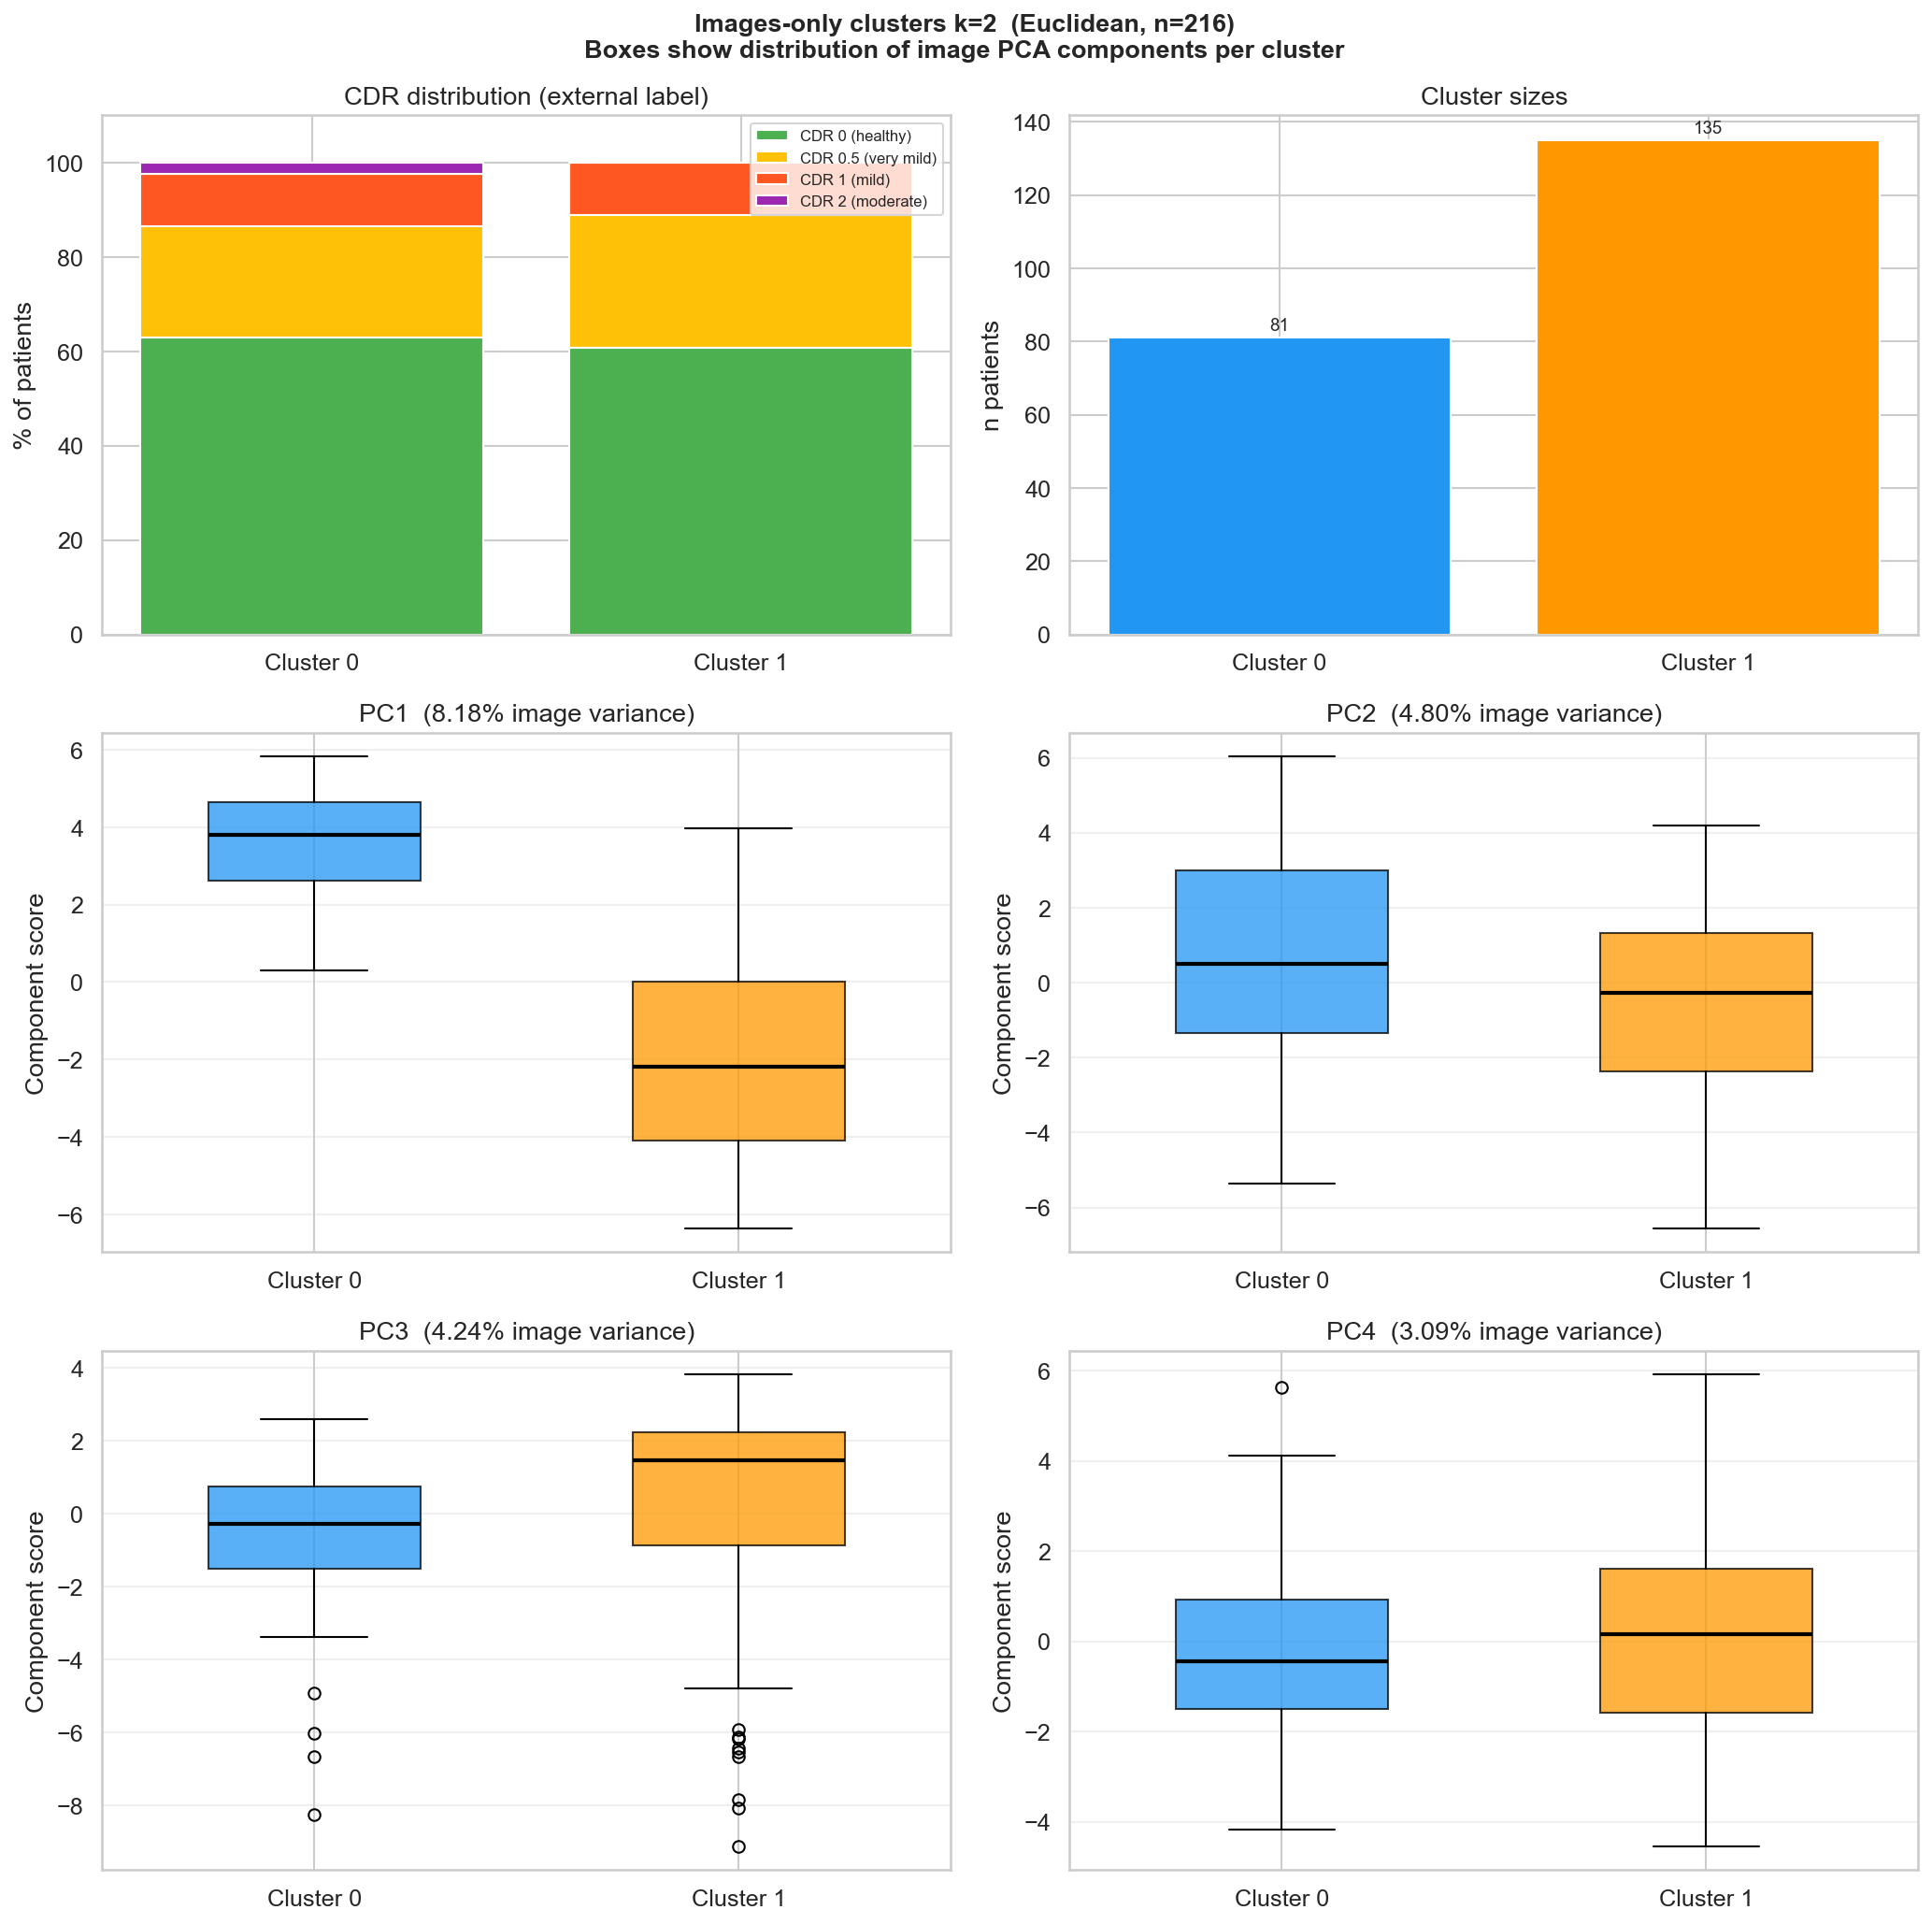
\includegraphics[width=\textwidth,height=0.42\textheight,keepaspectratio]{img_only_profile_k2.png}
        \caption{$k=2$}
    \end{subfigure}

    \begin{subfigure}[b]{\textwidth}
        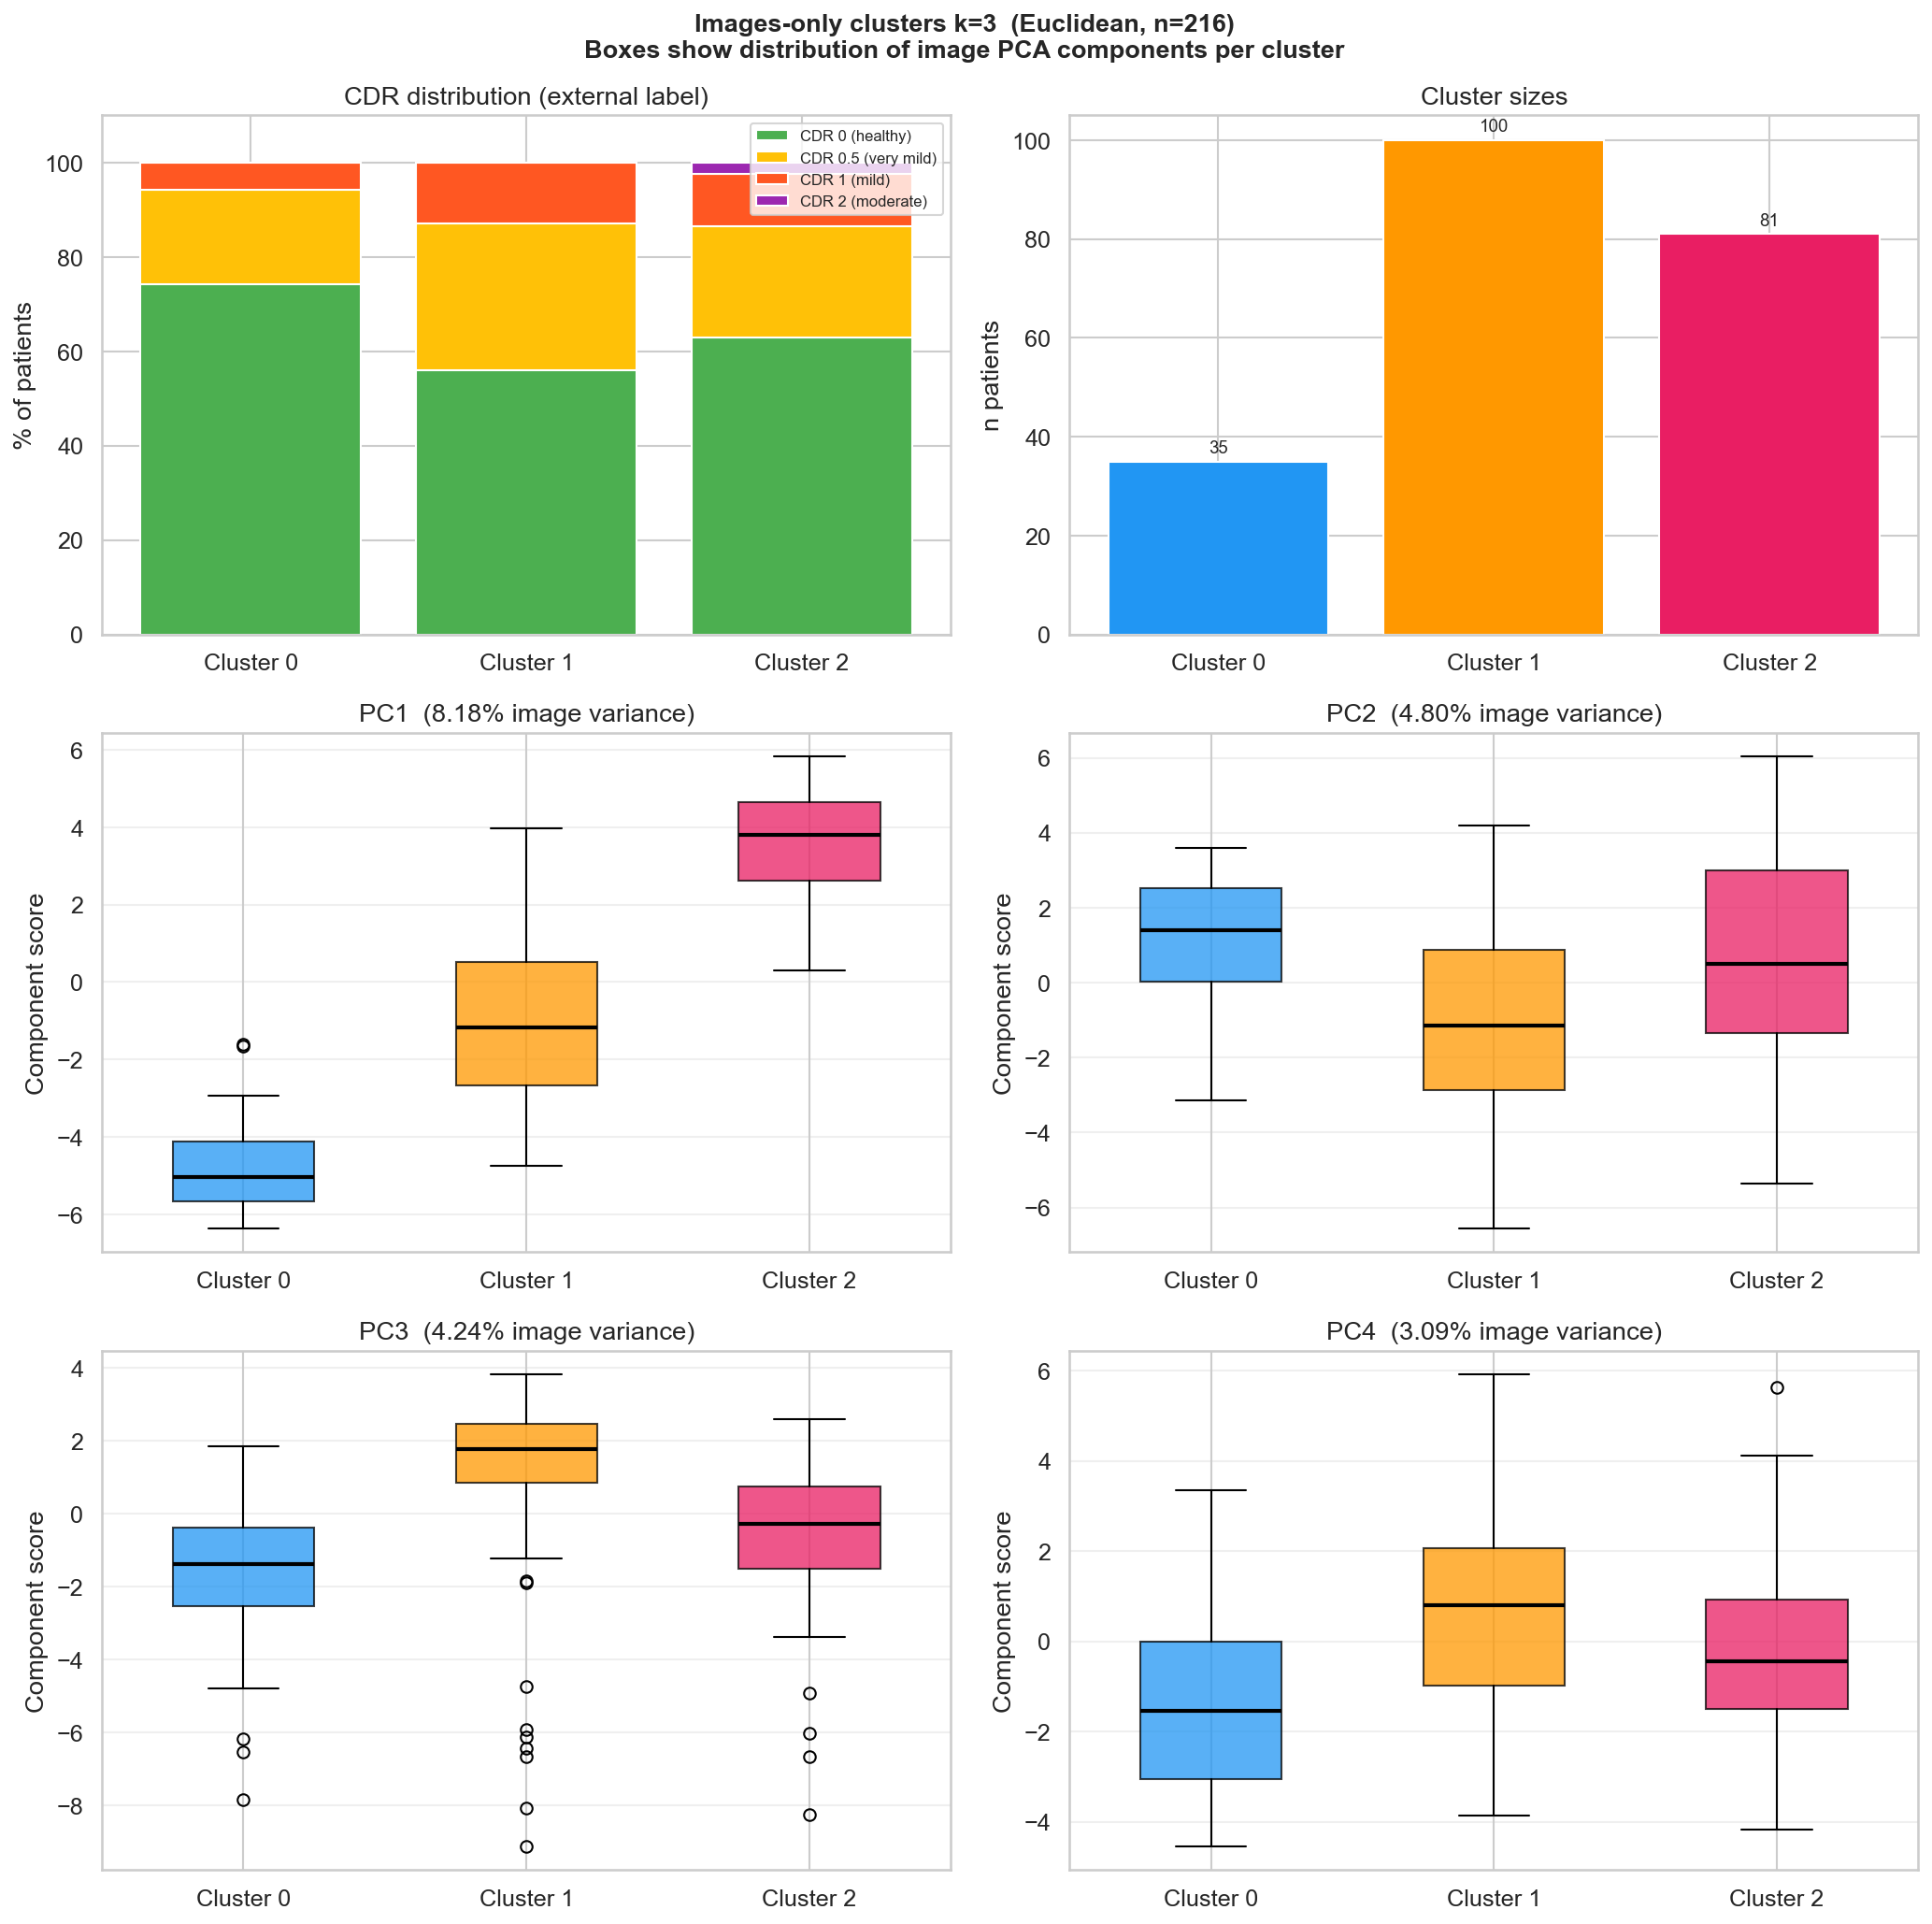
\includegraphics[width=\textwidth,height=0.42\textheight,keepaspectratio]{img_only_profile_k3.png}
        \caption{$k=3$}
    \end{subfigure}
    \caption{Cluster profiling — images only. Boxes show PC1–PC4 distributions per cluster.
    CDR (top-left) is an external label. The split is driven almost entirely by PC1.}
    \label{fig:img_profiles}
\end{figure}

\begin{figure}[H]
    \centering
    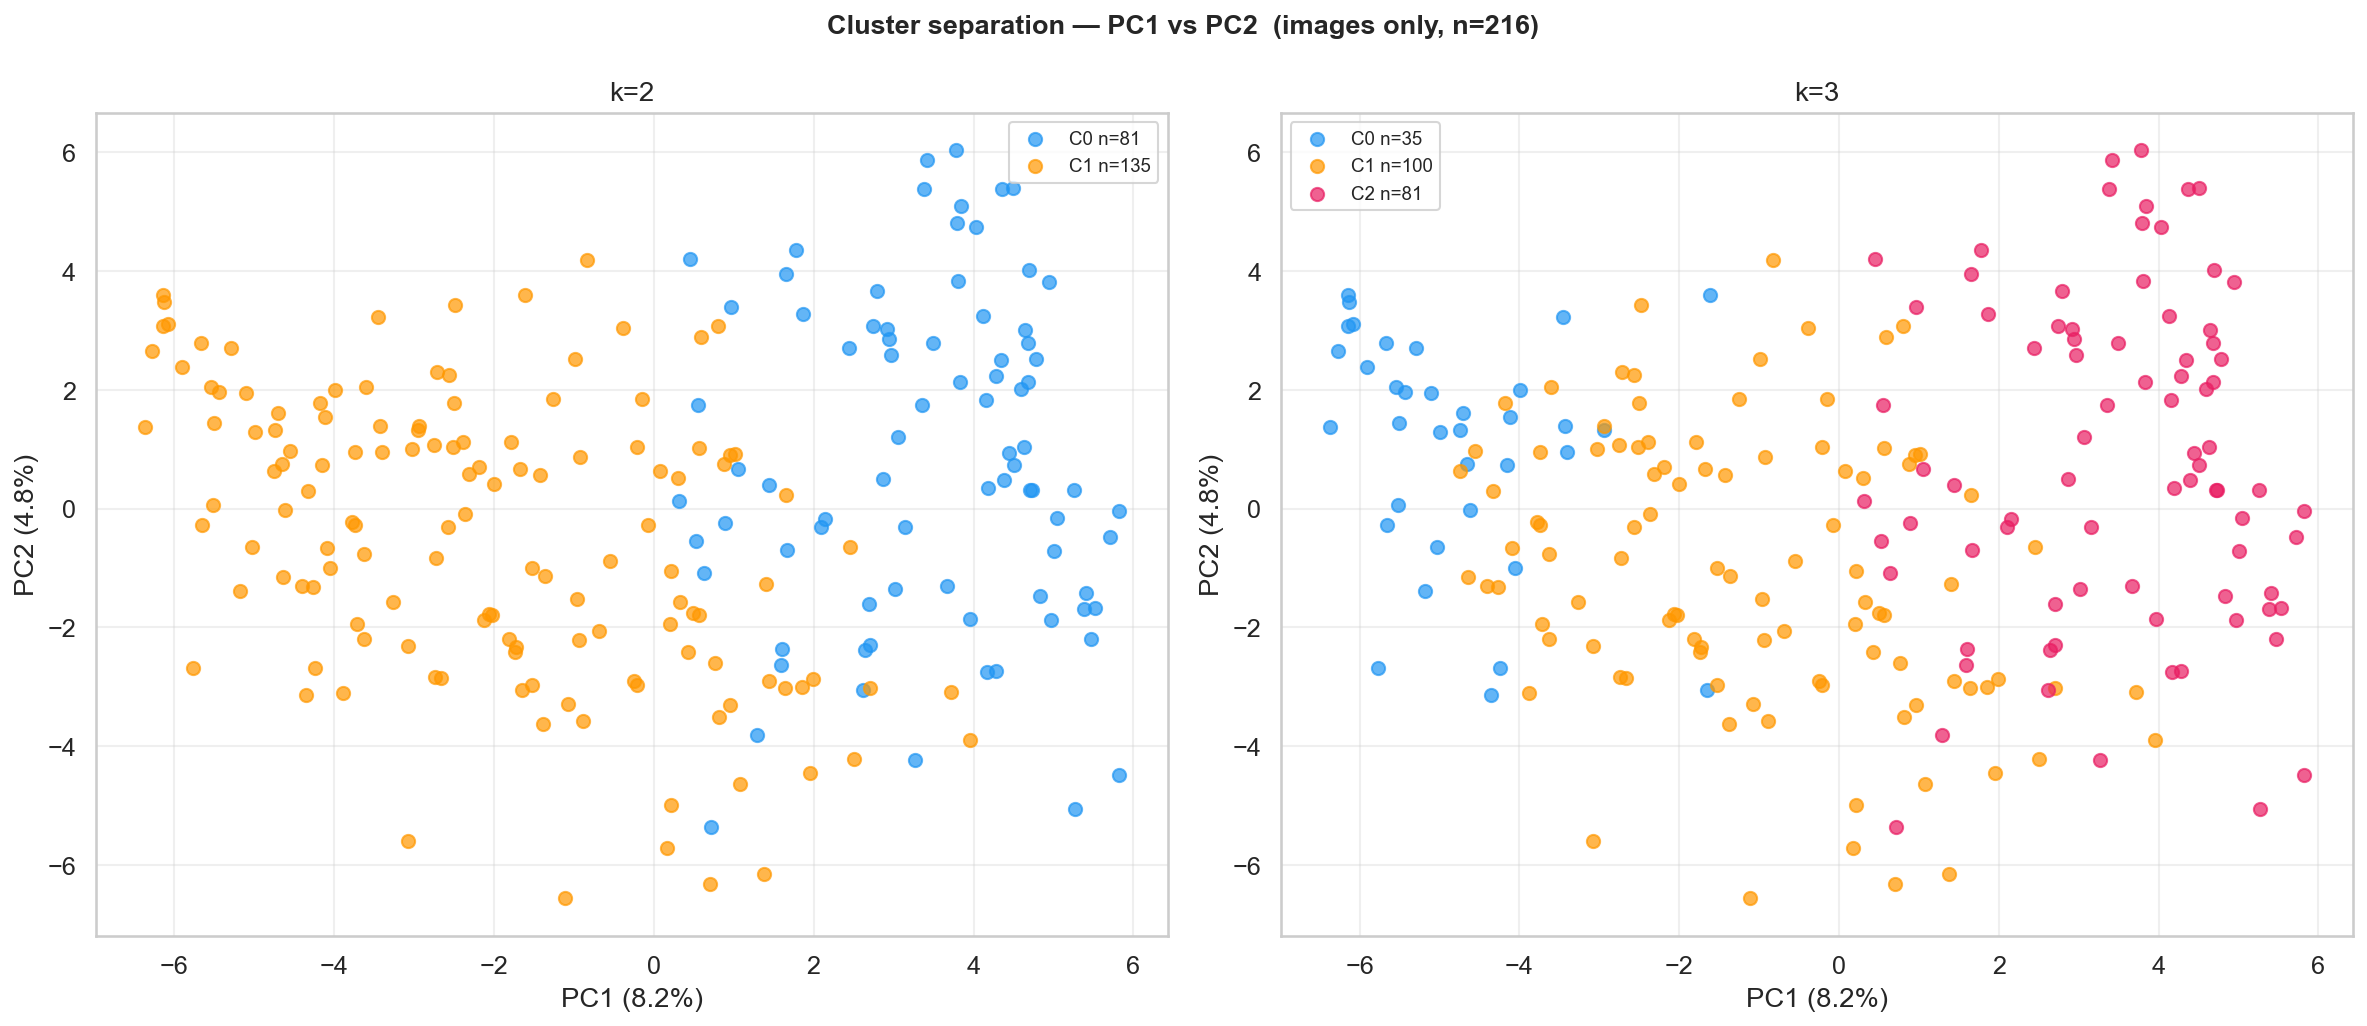
\includegraphics[width=0.9\textwidth]{img_only_pca_scatter.png}
    \caption{2D PCA scatter — images only. Variance is more evenly distributed
    across components than in clinical experiments (PC1=8.2\%, PC2=4.8\%).}
    \label{fig:img_pca2d}
\end{figure}

% ══════════════════════════════════════════════════════════════════════════════
\section{Experiment 4: Best Image Combination + Clinical}

\subsection{Configuration and Rationale}
\sloppy
Two image types are selected: \texttt{cor} (coronal, Talairach-registered) and
\texttt{gfc\_sag} (sagittal, Talairach-registered). This choice is motivated by:
\begin{itemize}[noitemsep]
    \item Two anatomically distinct views (different planes — no slice overlap)
    \item Both are globally registered to Talairach space, enabling fair comparison across patients
    \item Avoids known methodological issues: \texttt{sbj\_sag} is unregistered (native space);
    \texttt{masked\_tra} and \texttt{gfc\_tra} share the same anatomical slice (slice 90),
    with \texttt{masked\_tra} being the skull-stripped version of \texttt{gfc\_tra}
    (adding 45\% zero HOG features)
\end{itemize}

Feature matrix: $[\text{PCA}_\text{cor}\ |\ \text{PCA}_\text{gfc\_sag}\ |\ \text{clinical}]$.
Shape: $216 \times 228$. Distance: RelMS with $p_1 = [110, 110, 5]$, $p_3 = 3$.

\subsection{Evaluation}

\begin{table}[H]
\centering
\caption{Evaluation metrics — cor+gfc\_sag+clinical.}
\begin{tabular}{ccccc}
\toprule
$k$ & \textbf{Silhouette} & \textbf{ARI vs CDR} & \textbf{ARI vs Exp.\ 1} & Sizes \\
\midrule
2 & 0.0269 & 0.0320 & 0.6721 & 149 / 67 \\
3 & 0.0112 & 0.0161 & 0.5045 & 76 / 58 / 82 \\
\bottomrule
\end{tabular}
\end{table}

The ARI vs Experiment 1 (all 5 images + clinical) shows that using only two clean images
recovers 67\% of the patient groupings from the full 5-image experiment at $k=2$,
and 50\% at $k=3$.

\subsection{Cluster Profiles}

\textbf{$k=2$}:

\begin{table}[H]
\centering
\caption{Cluster profiles — cor+gfc\_sag+clinical, $k=2$.}
\begin{tabular}{lcc}
\toprule
\textbf{Feature} & \textbf{C0 ($n=149$)} & \textbf{C1 ($n=67$)} \\
\midrule
\% Female & \textbf{86.6\%} & 23.9\% \\
Age & $72.2 \pm 11.7$ & $72.9 \pm 13.6$ \\
MMSE & $27.3 \pm 3.5$ & $27.4 \pm 3.2$ \\
eTIV & $1379 \pm 96$ & $\mathbf{1635 \pm 132}$ \\
Education & $2.93 \pm 1.23$ & $3.90 \pm 1.32$ \\
SES & $2.73 \pm 1.03$ & $1.96 \pm 1.13$ \\
\midrule
CDR=0 & 65.1\% & 53.7\% \\
CDR=0.5 & 23.5\% & 32.8\% \\
CDR=1 & 10.7\% & 11.9\% \\
CDR=2 & 0.7\% & 1.5\% \\
\bottomrule
\end{tabular}
\end{table}

\textbf{$k=3$}:

\begin{table}[H]
\centering
\caption{Cluster profiles — cor+gfc\_sag+clinical, $k=3$.}
\begin{tabular}{lccc}
\toprule
\textbf{Feature} & \textbf{C0 ($n=76$)} & \textbf{C1 ($n=58$)} & \textbf{C2 ($n=82$)} \\
\midrule
\% Female & 75.0\% & 25.9\% & \textbf{89.0\%} \\
Age & $74.4 \pm 10.4$ & $71.4 \pm 14.4$ & $71.4 \pm 12.3$ \\
MMSE & $26.6 \pm 3.8$ & $27.7 \pm 3.0$ & $27.8 \pm 3.3$ \\
eTIV & $1429 \pm 94$ & $\mathbf{1650 \pm 129}$ & $1350 \pm 97$ \\
Education & $2.20 \pm 1.06$ & $\mathbf{4.24 \pm 1.10}$ & $3.48 \pm 1.02$ \\
SES & $3.32 \pm 1.00$ & $\mathbf{1.71 \pm 0.96}$ & $2.28 \pm 0.81$ \\
\midrule
CDR=0 & 52.6\% & 58.6\% & 72.0\% \\
CDR=0.5 & 27.6\% & 31.0\% & 22.0\% \\
CDR=1 & 18.4\% & 10.3\% & 4.9\% \\
CDR=2 & 1.3\% & 0.0\% & 1.2\% \\
\bottomrule
\end{tabular}
\end{table}

\subsection{Visualisations}

\begin{figure}[H]
    \centering
    \begin{subfigure}[b]{\textwidth}
        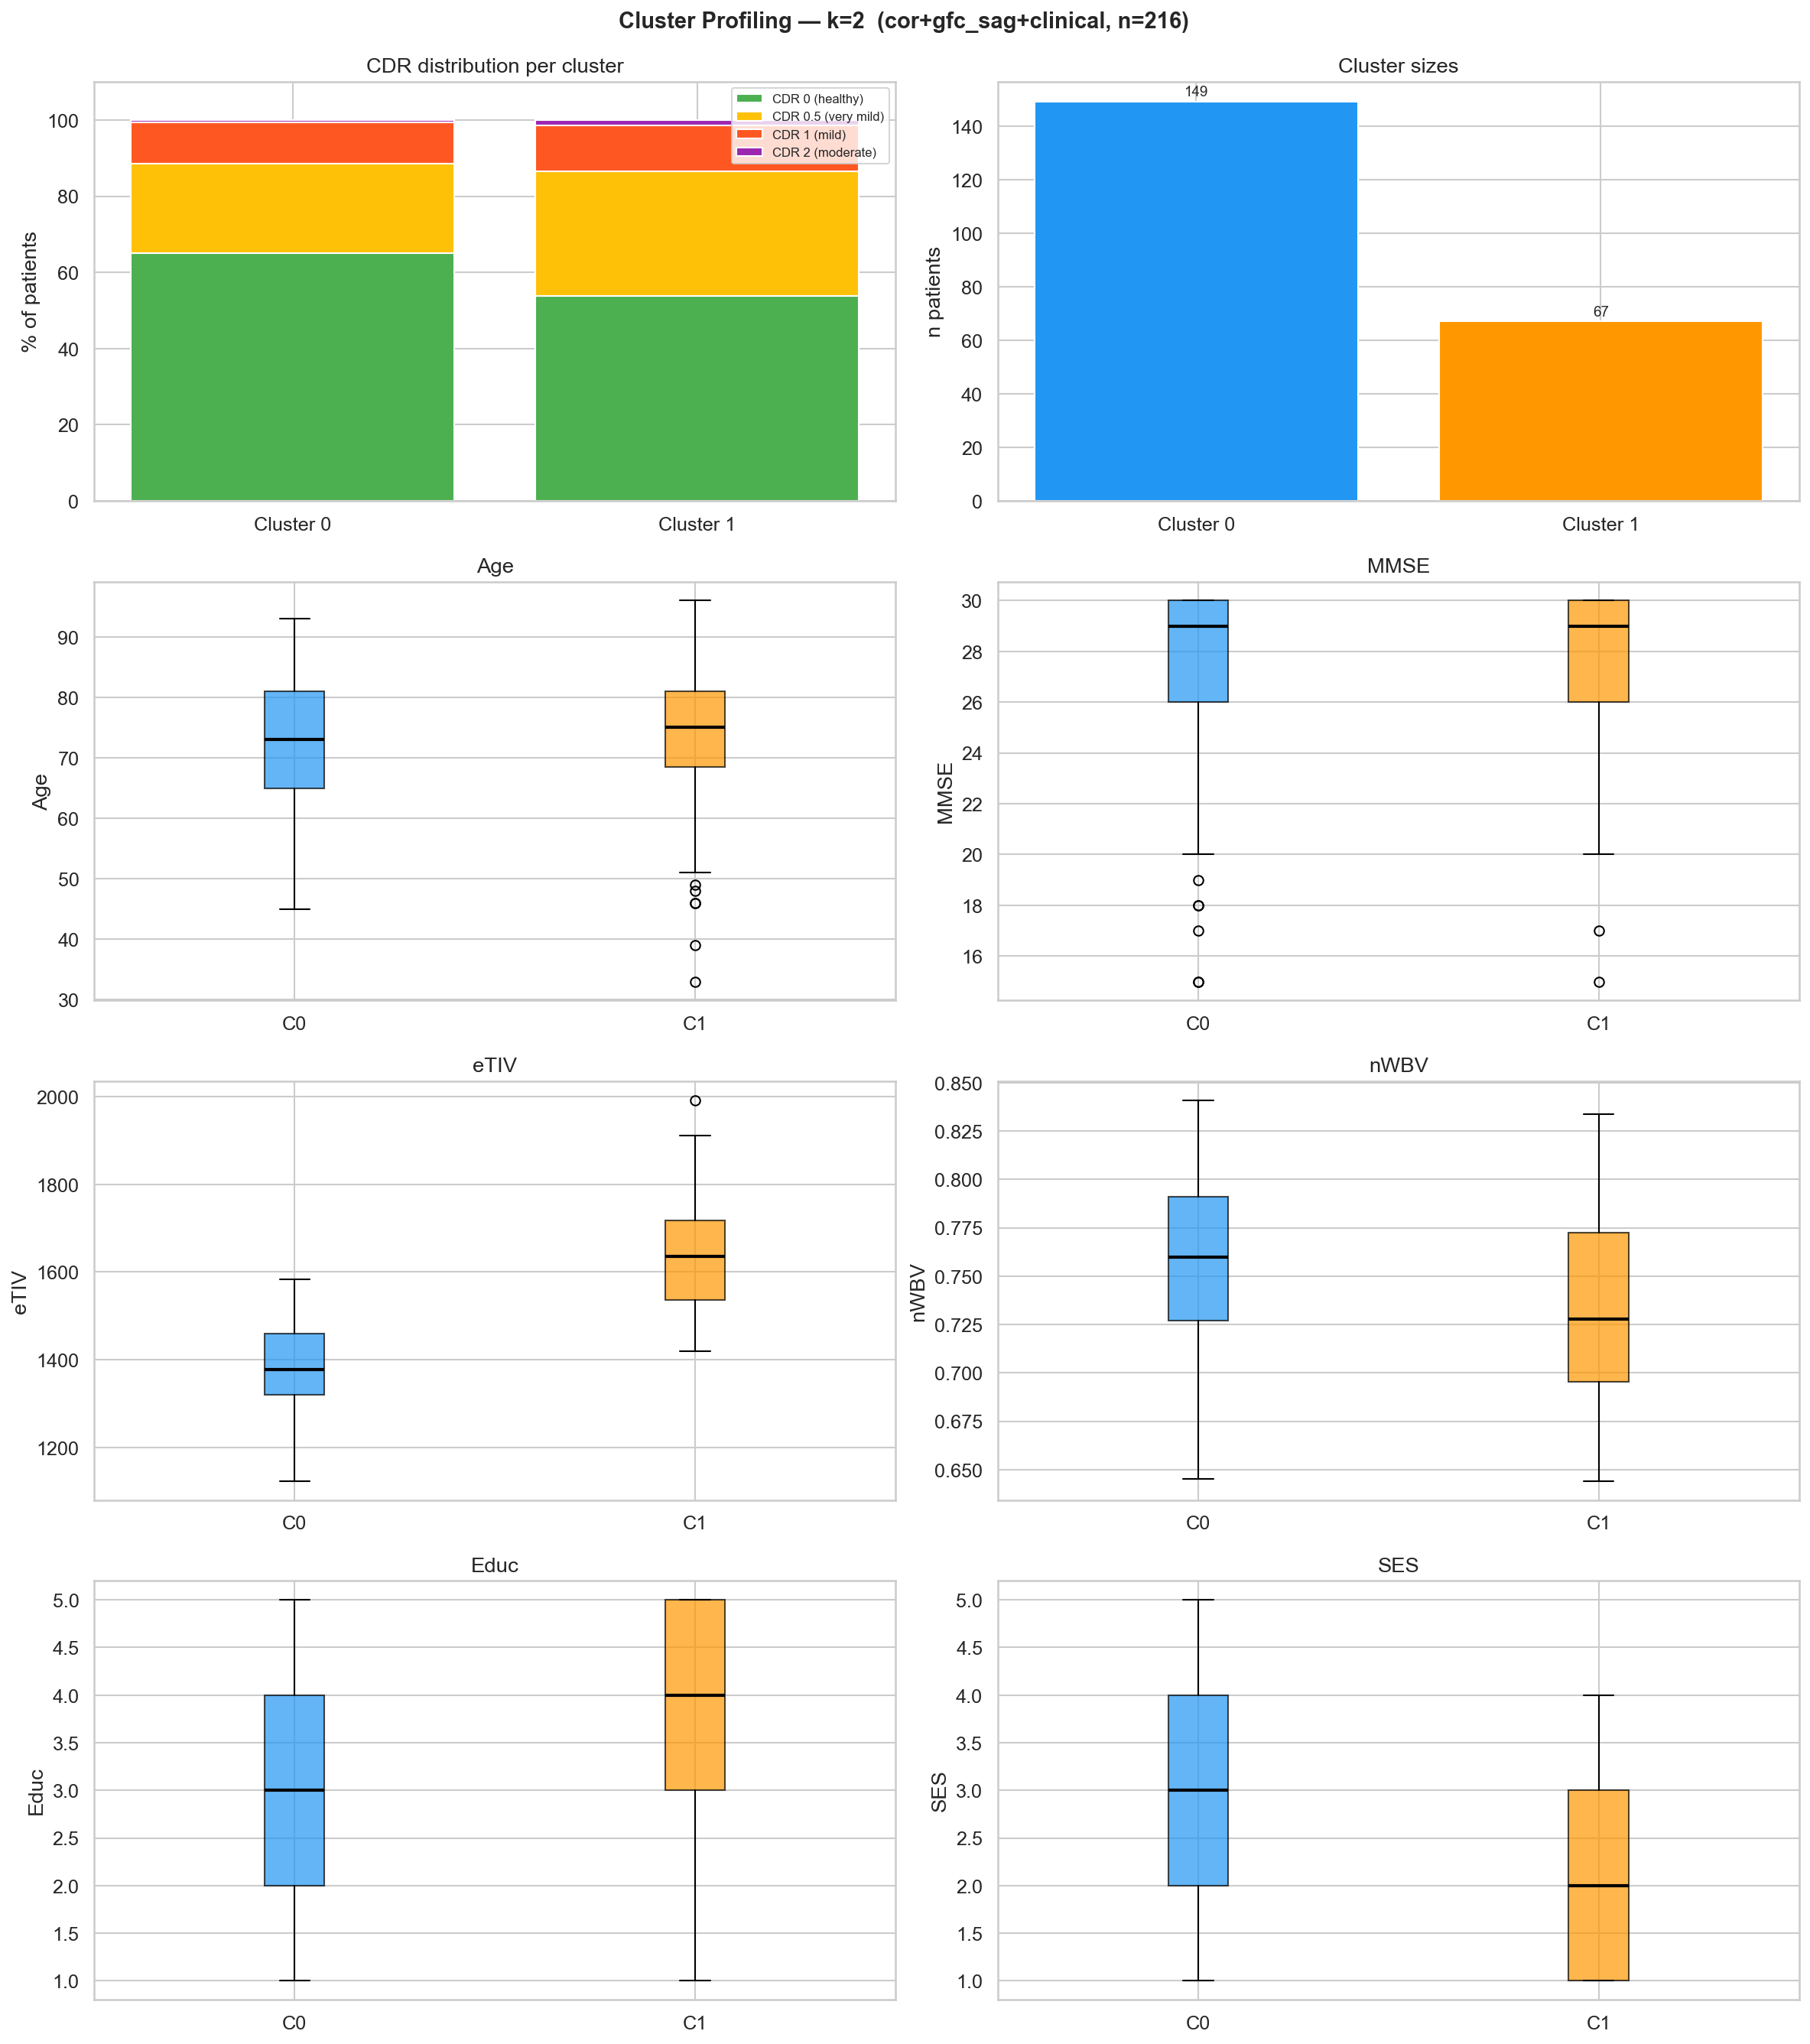
\includegraphics[width=\textwidth,height=0.42\textheight,keepaspectratio]{best_combo_profile_k2.png}
        \caption{$k=2$}
    \end{subfigure}

    \begin{subfigure}[b]{\textwidth}
        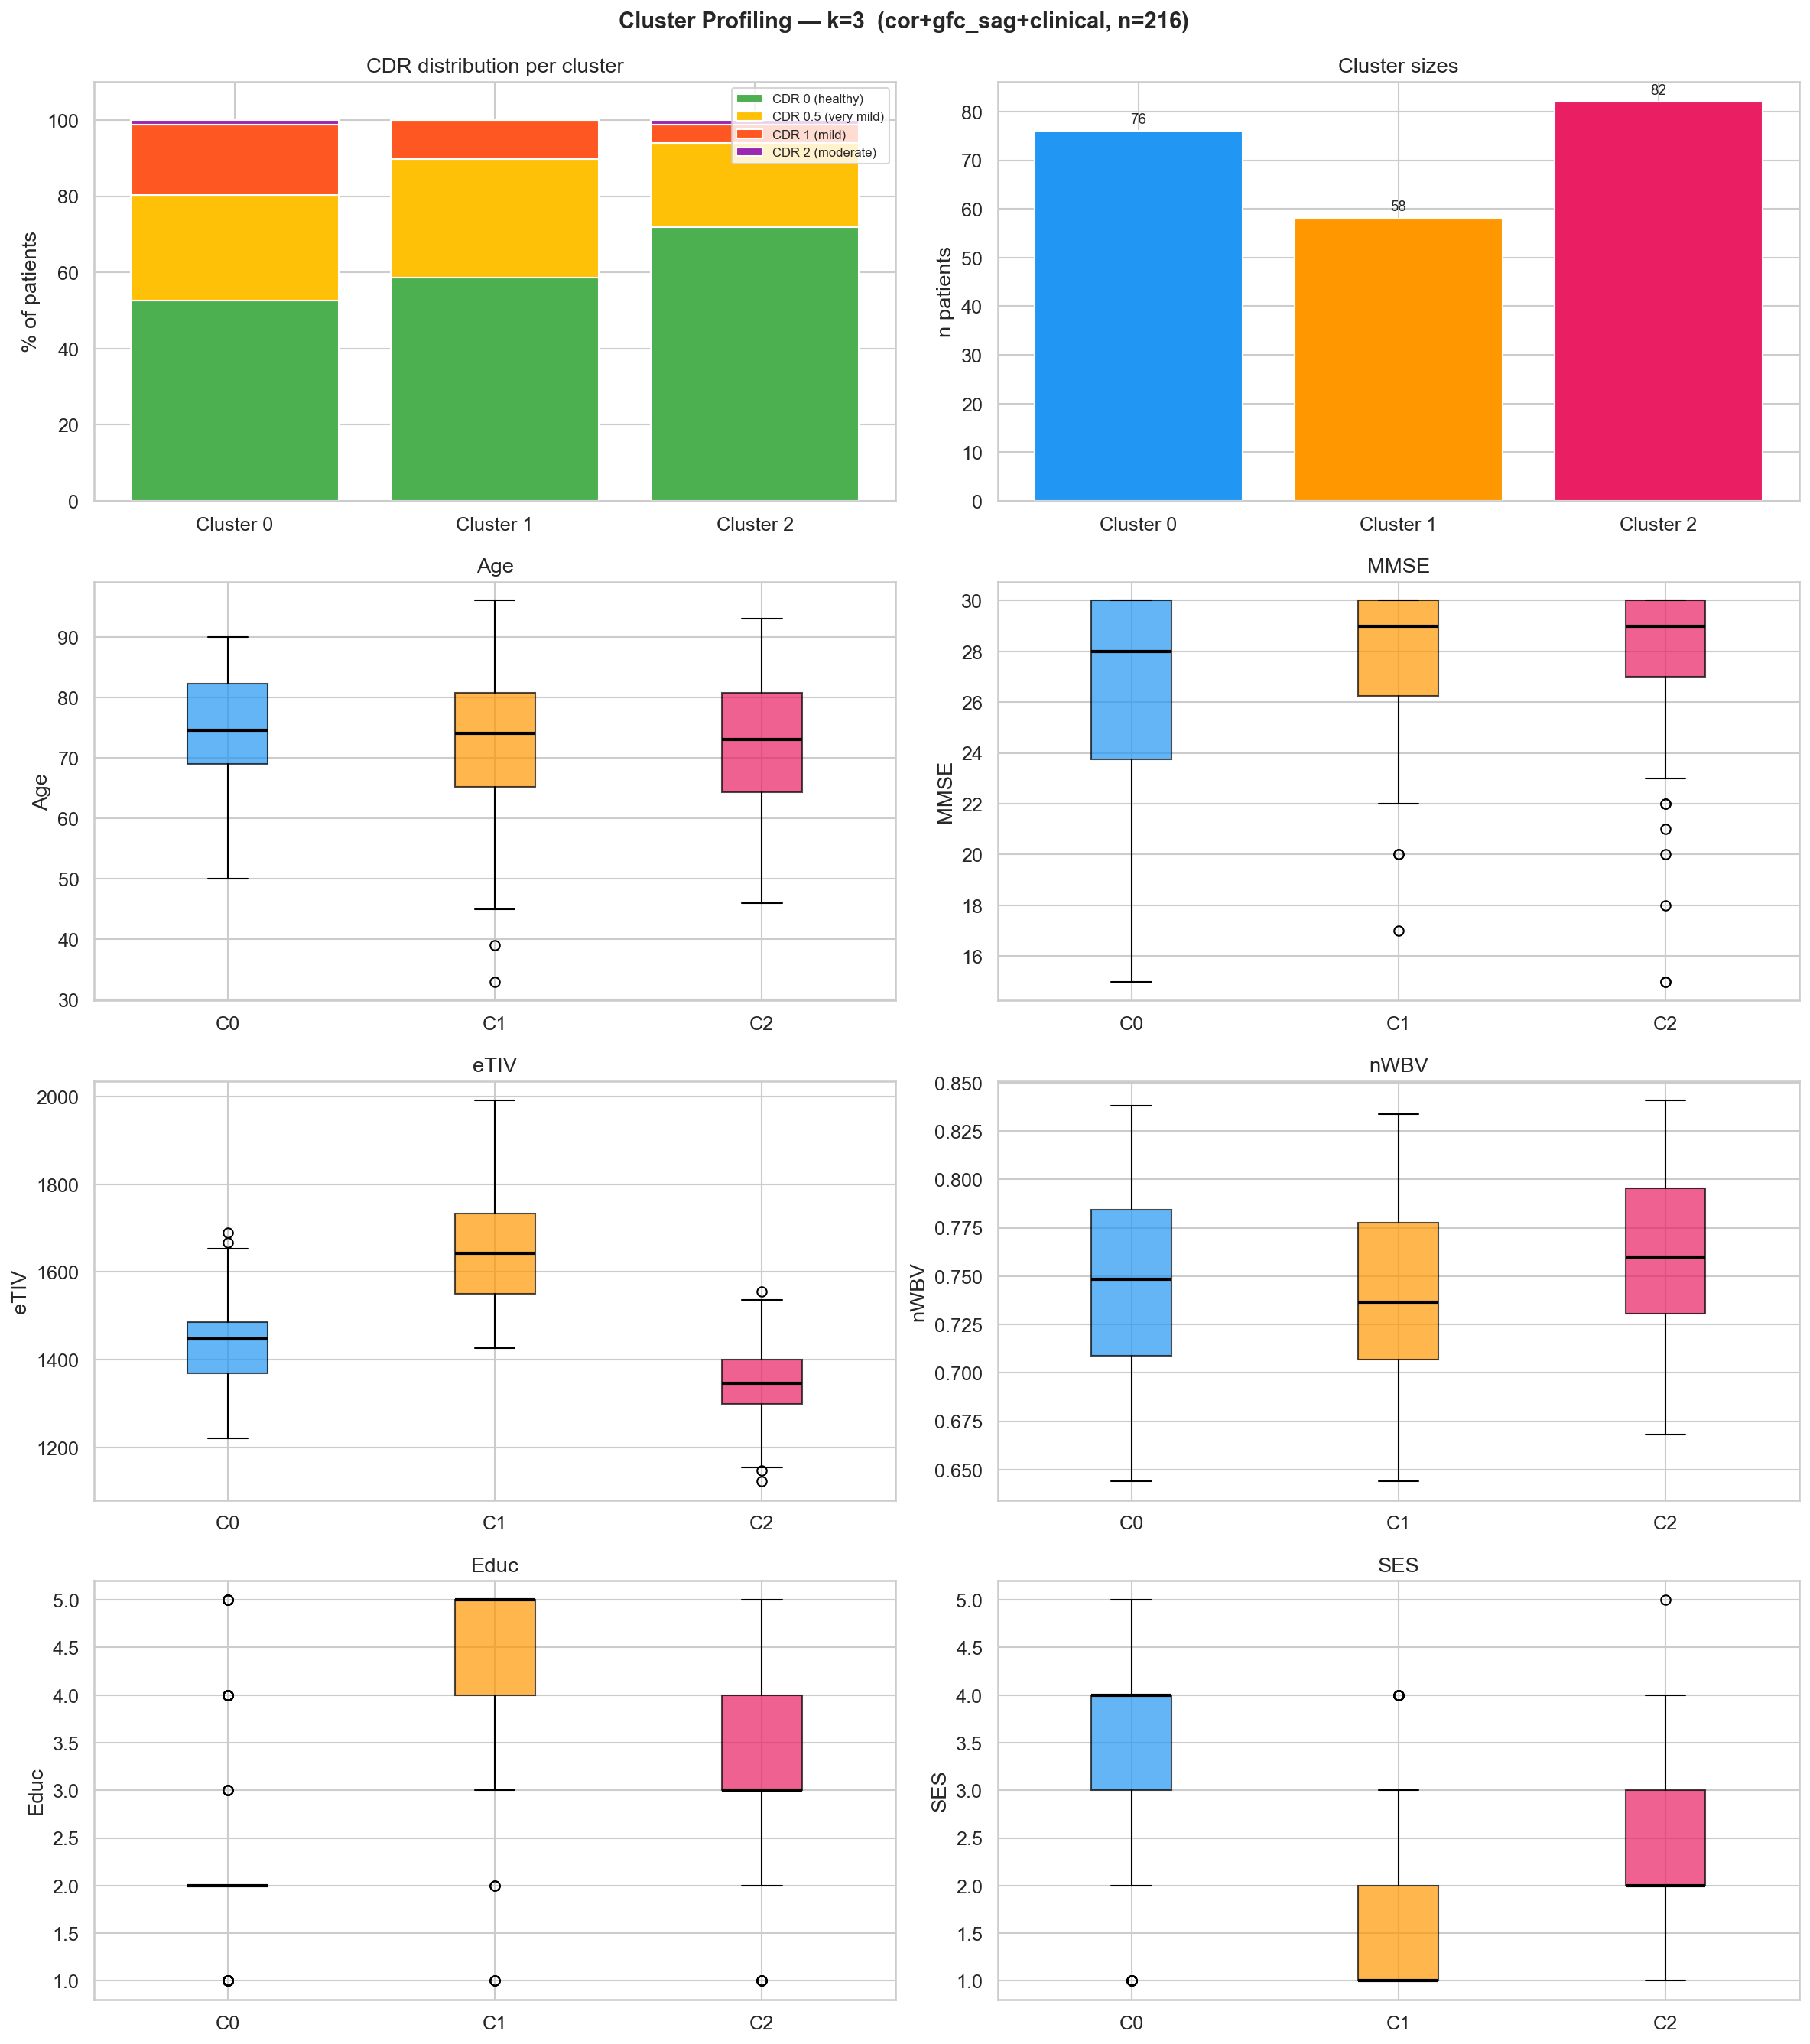
\includegraphics[width=\textwidth,height=0.42\textheight,keepaspectratio]{best_combo_profile_k3.png}
        \caption{$k=3$}
    \end{subfigure}
    \caption{Cluster profiling — cor+gfc\_sag + clinical.}
    \label{fig:best_profiles}
\end{figure}

\begin{figure}[H]
    \centering
    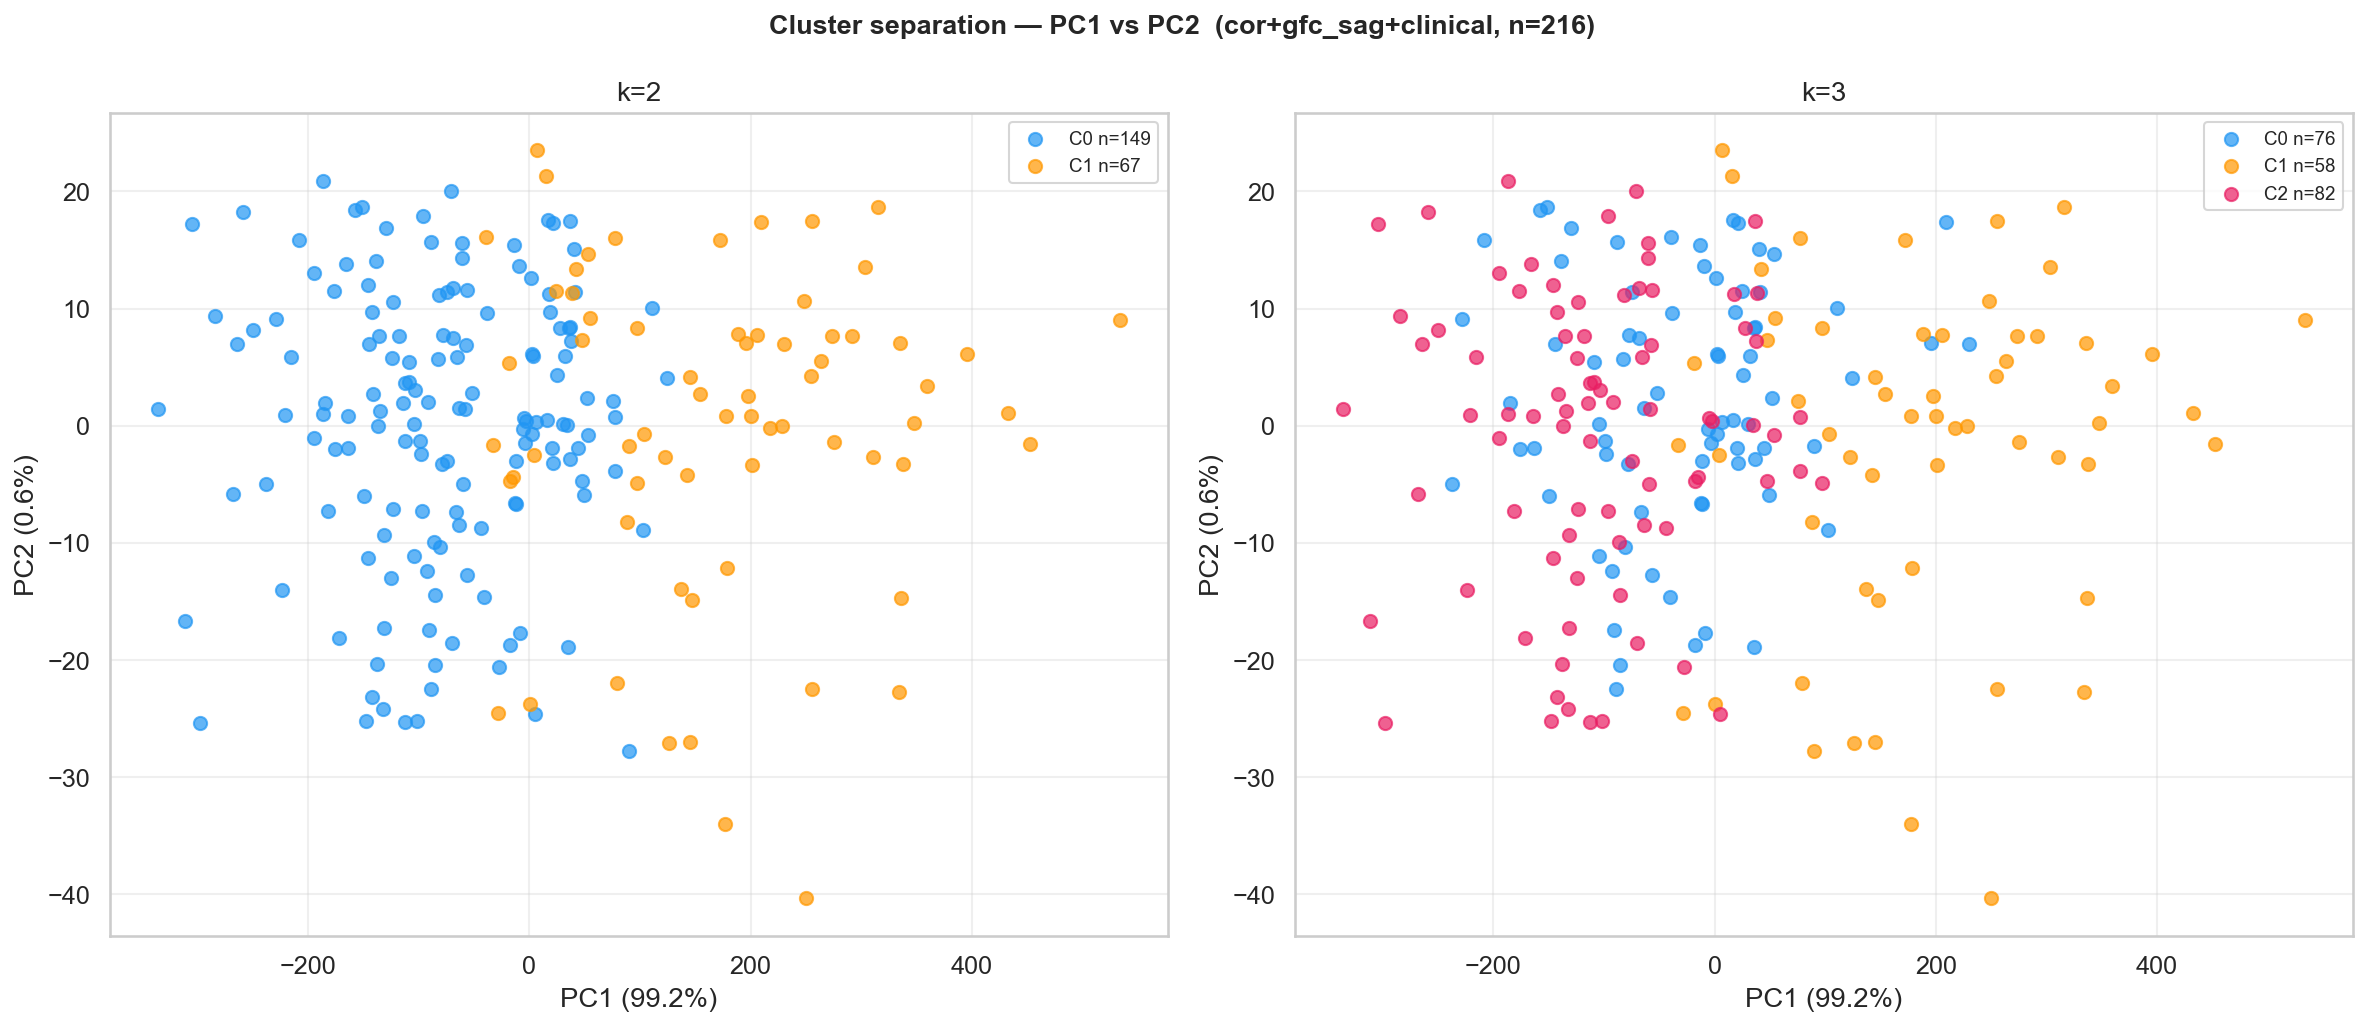
\includegraphics[width=0.9\textwidth]{best_combo_pca_scatter.png}
    \caption{2D PCA scatter — cor+gfc\_sag + clinical. PC1 = 99.2\%.}
    \label{fig:best_pca2d}
\end{figure}

\begin{figure}[H]
    \centering
    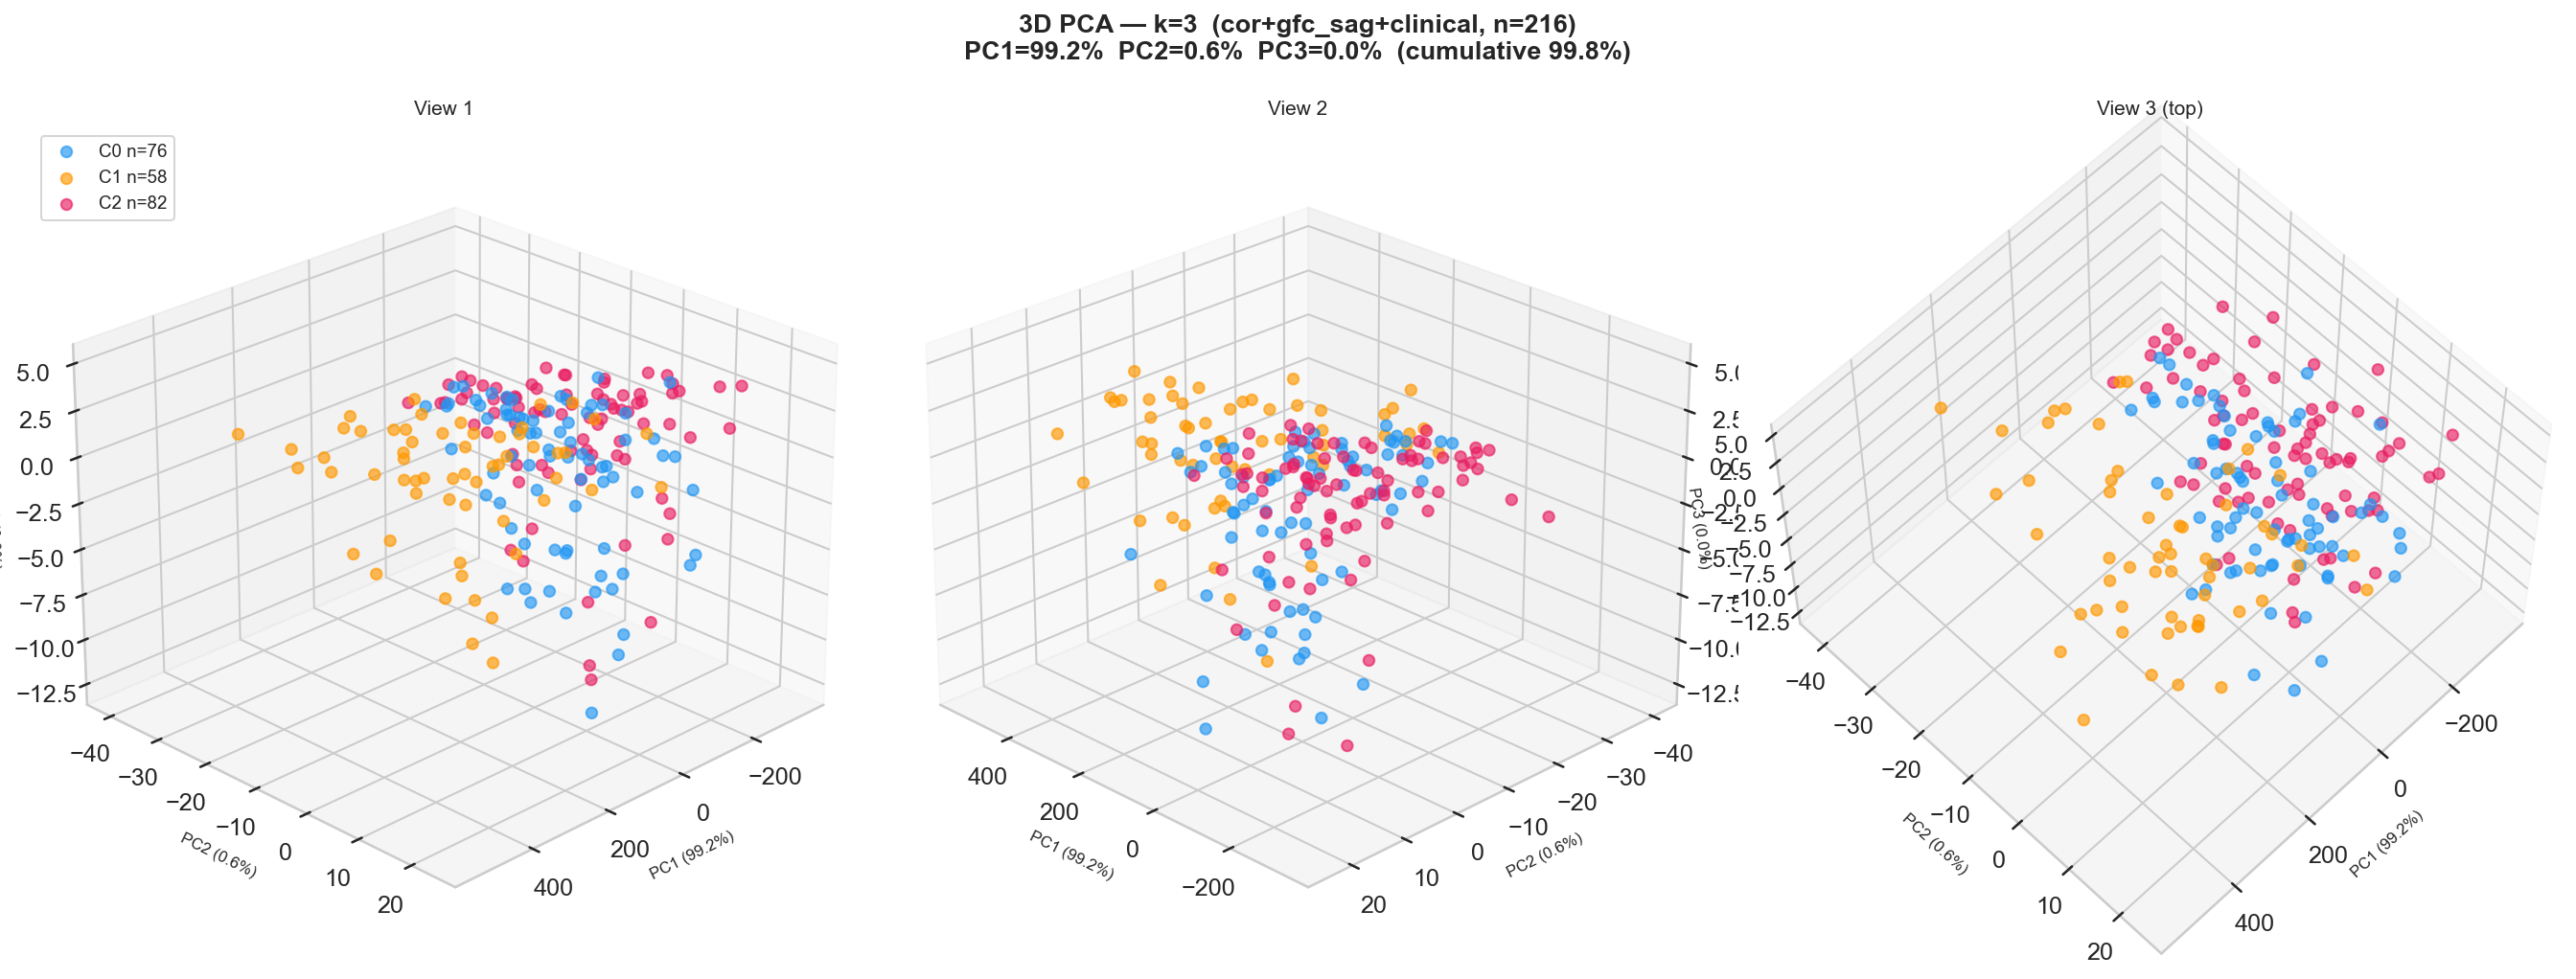
\includegraphics[width=\textwidth]{pca_3d_best_combo_k3.png}
    \caption{3D PCA scatter — cor+gfc\_sag+clinical, $k=3$.
    PC1=99.2\%, PC2=0.6\%, PC3=0.0\%. Same pattern as Experiments 1 and 2:
    the feature space is effectively 1-dimensional.}
    \label{fig:best_pca3d}
\end{figure}

% ══════════════════════════════════════════════════════════════════════════════
\section{Cross-Experiment Comparison}

\begin{table}[H]
\centering
\caption{Summary of all four experiments. Silhouette and ARI vs CDR for $k=2$ and $k=3$.
PC1 variance shows the effective dimensionality of each feature space.}
\renewcommand{\arraystretch}{1.2}
\begin{tabular}{lcccccc}
\toprule
& \multicolumn{2}{c}{\textbf{Silhouette}} &
  \multicolumn{2}{c}{\textbf{ARI vs CDR}} &
  \multicolumn{2}{c}{\textbf{PC1 variance}} \\
\cmidrule(lr){2-3}\cmidrule(lr){4-5}\cmidrule(lr){6-7}
\textbf{Experiment} & $k=2$ & $k=3$ & $k=2$ & $k=3$ & PC1 & PC2 \\
\midrule
All 5 images + clinical & 0.026 & 0.009 & 0.028 & 0.018 & 98.8\% & 0.6\% \\
Clinical only           & 0.029 & 0.013 & 0.025 & 0.018 & 99.4\% & 0.6\% \\
Images only             & 0.051 & 0.038 & $-$0.004 & $-$0.021 & 8.2\% & 4.8\% \\
cor+gfc\_sag+clinical   & 0.027 & 0.011 & 0.032 & 0.016 & 99.2\% & 0.6\% \\
\bottomrule
\end{tabular}
\end{table}

Key observations:
\begin{itemize}
    \item \textbf{All silhouette scores are very low ($< 0.06$)}: There is no strong natural
    cluster structure in this dataset at any tested $k$.

    \item \textbf{ARI vs CDR is near zero or negative in all experiments}: None of the
    discovered clusters correspond to CDR-defined disease stages.

    \item \textbf{Images only has the highest silhouette but the worst ARI}: More uniform
    Euclidean distances produce slightly tidier partitions, but those partitions have no
    clinical meaning.

    \item \textbf{Clinical data dominates all combined experiments}: The clinical-only and
    5-images+clinical experiments produce nearly identical cluster assignments. The
    cor+gfc\_sag+clinical configuration recovers 67\% of the full-set assignments at $k=2$,
    confirming the same dominance.

    \item \textbf{Feature space is effectively 1-dimensional wherever clinical data is used}:
    PC1 explains 98.8--99.4\% of variance in all clinical configurations, driven by eTIV.
    The 3D PCA visualisations confirm no additional structure in PC2 or PC3.
\end{itemize}

% ══════════════════════════════════════════════════════════════════════════════
\section{Feature Separation Between Clusters}

The evaluation metrics above (silhouette, ARI, NMI) answer \emph{how good} the clusters
are. This section answers a different and more informative question:
\textbf{which features actually differ between the clusters, and by how much?}
This is the practical output of the analysis --- it tells us what each cluster
\emph{is}, in terms of the original clinical variables.

\subsection{Method: Effect Sizes}

For each feature we compute an \textbf{effect size} that measures how strongly cluster
membership explains that feature's values. Unlike a raw mean difference, an effect size
is scale-free (0 to 1) so all features can be compared directly.

\begin{table}[H]
\centering
\caption{Effect-size measures used.}
\begin{tabular}{ll p{6.5cm}}
\toprule
\textbf{Measure} & \textbf{Feature type} & \textbf{Interpretation} \\
\midrule
$\eta^2$ (eta-squared) & Continuous / ordinal & Fraction of the feature's variance
   explained by the clusters \\
Cramér's V & Nominal (M/F) & Strength of association between feature and cluster \\
\bottomrule
\end{tabular}
\end{table}

The $\eta^2$ statistic is derived from the Kruskal--Wallis $H$ test:
\[
\eta^2 = \frac{H - k + 1}{n - k}
\]
where $k$ is the number of clusters and $n = 216$. The conventional interpretation is:
$\eta^2 \approx 0.01$ is a \emph{small} effect, $0.06$ is \emph{medium}, and
$0.14$ or above is a \emph{large} effect. Intuitively, $\eta^2 = 0.56$ for eTIV means
that 56\% of the variation in brain volume is explained purely by which cluster a patient
belongs to --- an extremely strong separation.

\subsection{Result: Which Features Drive the Clustering}

Figure~\ref{fig:eta2_heatmap} is the central result of this section. Each cell shows the
$\eta^2$ of one clinical feature (row) in one experiment (column). Darker red means the
feature differs more strongly between the clusters.

\begin{figure}[H]
    \centering
    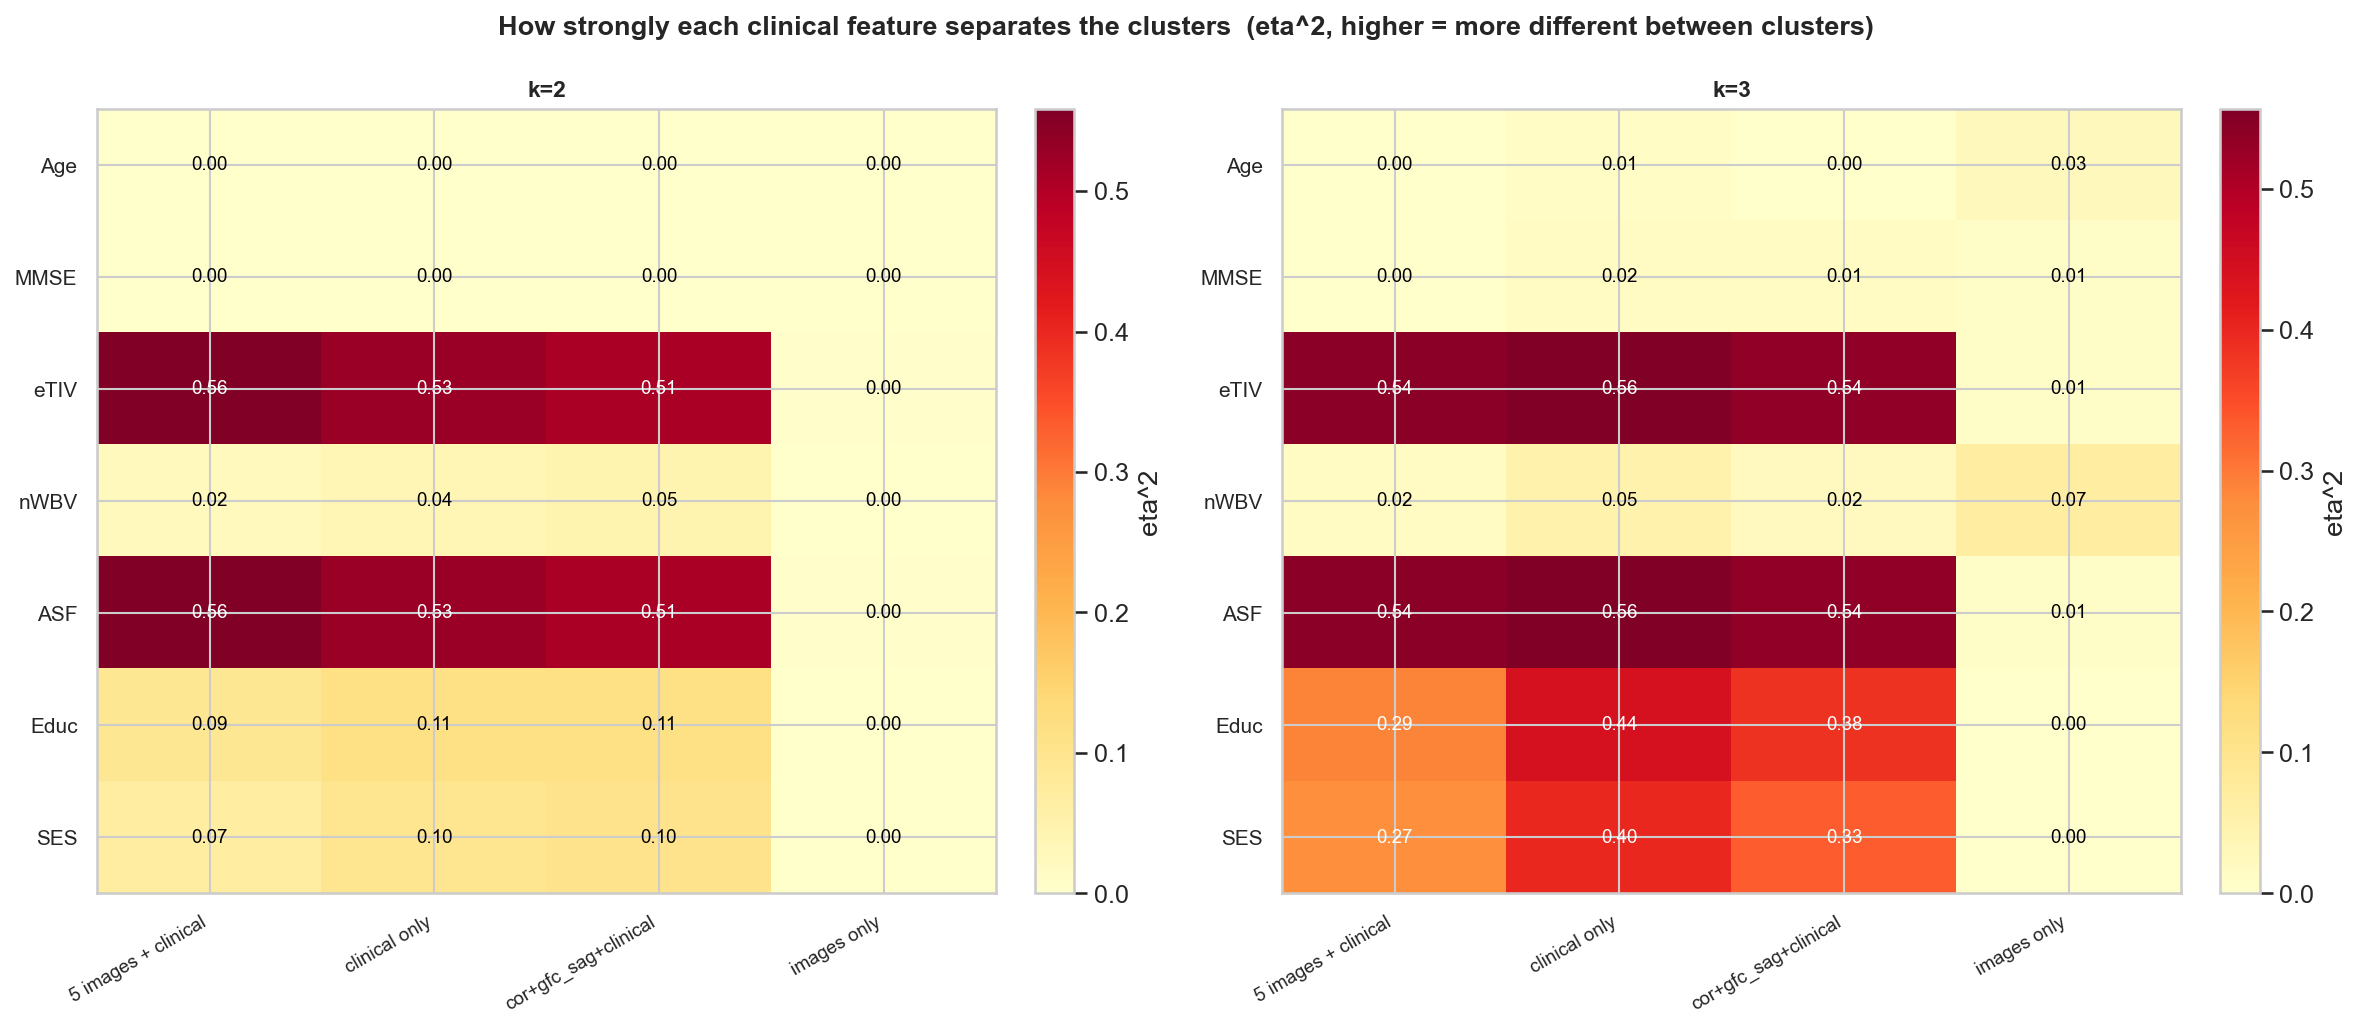
\includegraphics[width=\textwidth]{feature_separation_eta2.png}
    \caption{Feature separation ($\eta^2$) of each clinical feature across all four
    experiments, at $k=2$ (left) and $k=3$ (right). Darker = the feature differs more
    strongly between clusters. For the \emph{images only} column these values are
    \textbf{external} (the clinical features were never used in that clustering), so they
    reveal whether image-derived clusters accidentally recover any clinical structure.}
    \label{fig:eta2_heatmap}
\end{figure}

Table~\ref{tab:eta2_full} gives the exact numbers, ranked, including the nominal M/F
feature (Cramér's V) and the external CDR alignment.

\begin{table}[H]
\centering
\caption{Effect sizes of every feature in every experiment. M/F uses Cramér's V;
all others use $\eta^2$. CDR is an external label (never used in clustering).
Bold = large effect ($\geq 0.14$).}
\renewcommand{\arraystretch}{1.15}
\setlength{\tabcolsep}{4pt}
\small
\begin{tabular}{l cc cc cc cc}
\toprule
& \multicolumn{2}{c}{\textbf{5 img + clin}}
& \multicolumn{2}{c}{\textbf{clinical only}}
& \multicolumn{2}{c}{\textbf{cor+gfc\_sag}}
& \multicolumn{2}{c}{\textbf{images only}} \\
\cmidrule(lr){2-3}\cmidrule(lr){4-5}\cmidrule(lr){6-7}\cmidrule(lr){8-9}
\textbf{Feature} & $k{=}2$ & $k{=}3$ & $k{=}2$ & $k{=}3$ & $k{=}2$ & $k{=}3$ & $k{=}2$ & $k{=}3$ \\
\midrule
M/F (sex)  & \textbf{.64} & \textbf{.56} & \textbf{.63} & \textbf{.59} & \textbf{.61} & \textbf{.55} & \textbf{.14} & \textbf{.17} \\
eTIV       & \textbf{.56} & \textbf{.54} & \textbf{.53} & \textbf{.56} & \textbf{.51} & \textbf{.54} & .00 & .01 \\
ASF        & \textbf{.56} & \textbf{.54} & \textbf{.53} & \textbf{.56} & \textbf{.51} & \textbf{.54} & .00 & .01 \\
Educ       & .09 & \textbf{.29} & .12 & \textbf{.44} & .11 & \textbf{.38} & .00 & .00 \\
SES        & .07 & \textbf{.27} & .10 & \textbf{.40} & .10 & \textbf{.33} & .00 & .00 \\
nWBV       & .02 & .02 & .04 & .05 & .05 & .02 & .00 & \textbf{.07} \\
Age        & .00 & .00 & .00 & .01 & .00 & .00 & .00 & .03 \\
MMSE       & .00 & .00 & .00 & .02 & .00 & .01 & .00 & .01 \\
\midrule
CDR (ext.) & .13 & .14 & .10 & \textbf{.17} & .12 & \textbf{.16} & .13 & .13 \\
\bottomrule
\end{tabular}
\label{tab:eta2_full}
\end{table}

\subsection{Interpretation}

Reading the heatmap and table together gives a clear and consistent story:

\begin{itemize}
    \item \textbf{Sex and brain volume dominate every clustering.} M/F
    (Cramér's V $\approx 0.55$--$0.64$), eTIV and ASF ($\eta^2 \approx 0.51$--$0.56$)
    are \emph{large} effects in all three experiments that use clinical data. The clusters
    are, first and foremost, a split between smaller-brained females and larger-brained males.

    \item \textbf{ASF and eTIV are identical} because they are mathematically redundant
    ($\text{ASF} = 1.2109/\text{eTIV}^{1/3}$). They always have the same $\eta^2$, which
    effectively double-counts brain volume in the distance metric.

    \item \textbf{Age and MMSE never separate the clusters} ($\eta^2 \approx 0.00$).
    These are the two features most directly related to cognitive decline, yet the
    clustering is completely blind to them. This is the clearest evidence that the
    clusters are demographic, not disease-related.

    \item \textbf{Education and SES only matter at $k=3$.} At $k=2$ they are small
    ($\eta^2 \approx 0.07$--$0.12$), but at $k=3$ they become large
    ($\eta^2 \approx 0.27$--$0.44$). This tells us exactly what the third cluster is:
    when the algorithm is forced to find a third group, it splits patients by
    socioeconomic status, not by disease.

    \item \textbf{Images carry no clinical signal.} The entire \emph{images only} column
    is near zero for every clinical feature ($\eta^2 \approx 0.00$). Even though these
    clusters were built from 550 image features, they fail to recover brain volume, sex,
    education, or any clinical variable. The HOG image features do not encode the
    demographic or clinical structure of the patients.

    \item \textbf{CDR alignment is weak everywhere.} The external CDR row stays around
    $0.10$--$0.17$ (weak association). It nudges just past the ``large'' threshold only for
    clinical-only and cor+gfc\_sag at $k=3$ --- the same two configurations where
    education/SES became strong --- but never reaches a level that would support using the
    clusters to predict disease stage.
\end{itemize}

For completeness, the images-only clusters were also profiled by their own image PCA
components. At $k=3$, principal component~1 has $\eta^2 = 0.74$ (very large) and
component~3 has $\eta^2 = 0.32$, while components 2, 4, and 5 are small. The image
clustering is therefore essentially a split along a single dominant image direction (PC1),
which most likely encodes global brain size and shape --- the same information that eTIV
already provides in the clinical data.

\end{document}

